\UseRawInputEncoding
\chapter{Implementation}
I will be implementing my project using Microsoft Visual Studio 2019 within a Windows Executable application template using the .NET Core framework version 3.1. \newline
The first form I will design is the main menu as this is what the players will see first when they open the game.

\section{Designing the Main Menu}
I began by setting up the form background colour then added the panel controls then I added the rest of the controls to the screen. I made sure to give all the controls which would have events associated to them in the code a meaningful name, to ensure I could address them without confusion of which control was which. For example, the button which loads a new game is called \verb|btnNewGame| (screenshots of the forms annotated with the control names are available in Appendix \ref{app:ScreenshotsOfForms}).\\
I also made sure that the controls on the forms responded dynamically to the size of the window to make sure that as the window was resized, the controls would move to the centre.
The final main menu form (design) is shown below:
\begin{figure}[H]
    \centering
    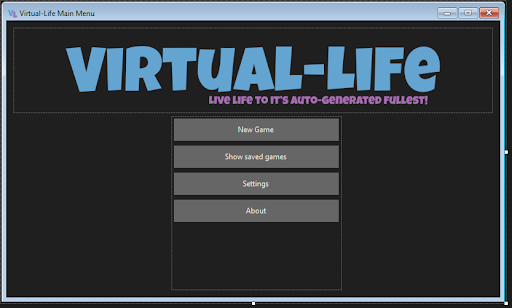
\includegraphics[width=0.8\textwidth]{images/implementation/mainMenu.png}
    \caption{Main menu form design}
    \label{fig:implementation-mainMenu}
\end{figure}

\section{Declaring Classes and Passing Objects Between Forms}
Now that I have a basic user interface (UI) designed, I am able to begin programming the game which will run behind it. I will start with moving an object between forms. This is fundamental to my game as I will be constructing an object in one form then moving it to another form where it will be processed. It is important that the object along with all its attributes is moved in its entirety. This means that as the game progresses from the new game screen to the main game play form, the objects already generated are accessible. \newline
To work out how to do this was quite a complicated process as there were lots of different out of date tutorials on the internet, it taught me the importance of testing small elements of the code in a test project before moving them into the main program.
\begin{lstlisting}[language=c, style=csharp, caption=Displaying a new form and passing an object to it]
frmMainGameScreen fMainGameScreen = new frmMainGameScreen(mainCharacter); //create new frmMainGameScreen with parameter mainCharacter
fMainGameScreen.Show(); //show new main game screen.
\end{lstlisting}
\noindent The code above creates the new instance for \verb|frmMainGameScreen| and passes into the constructor the \verb|mainCharacter| object. The \verb|mainCharacter| object is passed from form to form throughout the program.\\
The code below takes the object (being passed into the new form) as a parameter of the constructor of the form.
\begin{lstlisting}[language=c, style=csharp, caption=New form constructor code containing processing for object being passed in as a parameter]
public frmMainGameScreen(Person mainCharacterTransfer)
{
    InitializeComponent();            
    mainCharacter = mainCharacterTransfer; //Set the contents of mainCharacter to mainCharacterTransfer which has come from previous form
}
\end{lstlisting}

\section{Creating the Person classes}
Using my class diagrams, I then setup the rest of the classes and setup the inheritance for the classes relating to people. For now, I have only inputted the attributes for the classes, methods will be setup later as I need them.
\begin{lstlisting}[language=c, style=csharp, caption=GenericFamilyMember class creation]
 public class GenericFamilyMember : Person
{
    private string relationshipToMain;

    //get and set
    public string RelationshipToMain { get; set; }
}
\end{lstlisting}
\begin{lstlisting}[language=c, style=csharp, caption=MainCharacter class creation]
public class MainCharacter : DetailedCharacter
{
    //attributes

    private int expenses;
    private int bankBalance;
    private int jobBand;
    private string jobTitle;
    private int jobSalary;
    private int jobCurrentDuration;
    private int salary;

    //get and set
    public int Expenses { get; set; }
    public int BankBalance { get; set; }
    public int JobBand { get; set; }
    public string JobTitle { get; set; }
    public int JobSalary { get; set; }
    public int JobCurrentDuration { get; set; }
}
\end{lstlisting}
\begin{lstlisting}[language=c, style=csharp, caption=Partner class creation]
public class Partner : DetailedCharacter
{
    Random rnd = new Random();
    private string whereMet;
    private DateTime whenMet;

    //get and set
    public string WhereMet { get; set; }
    public DateTime WhenMet { get; set; }
}
\end{lstlisting}
\begin{lstlisting}[language=c, style=csharp, caption=Person class creation]
public class Person
    {
        //Set all private attributes for the class
        private string firstName;
        private string lastName;
        private string gender;
        private string sexuality;
        private int age;
        private bool livingStatus;
        private DateTime dateOfBirth;
        private DateTime dateOfDeath;
        private string reasonForDeath;
        private bool inRelationship;
        //get and set methods (nb. use uppercase first character for accessable get/set)
        public string FirstName { get; set; }
        public string LastName { get; set; }
        public string Gender { get; set; }
        public string Sexuality { get; set; }
        public int Age { get; set; }
        public bool LivingStatus { get; set; }
        public DateTime DateOfBirth { get; set; }
        public DateTime DateOfDeath { get; set; }
        public string ReasonForDeath { get; set; }
        public bool InRelationship { get; set; }
    }
\end{lstlisting}
\section{Working More on The Forms}
Now I had the basics worked out (how to pass data from one form to another and accessing objects in C\#), I designed the new game and show saved games form. Both of these forms are fundamentally the same, with each having text boxes for the attributes of the main character. However, on the show saved games form, the text boxes are read only and they get populated once the user has opened the file.
\begin{figure}[H]
    \centering
    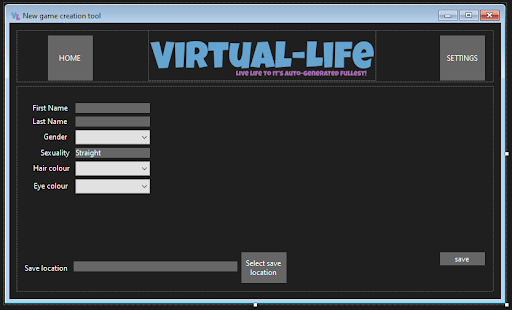
\includegraphics[width=0.8\textwidth]{images/implementation/newGameForm.png}
    \caption{Create new game form}
    \label{fig:implementation-newGameForm}
\end{figure}
\noindent The figure below shows the show saved games form. It contains text box controls which will be used to show the main characters information to the player, this will allow them to confirm that they have selected the correct save before the computer loads the data then then the game progresses to the next form.
\begin{figure}[H]
    \centering
    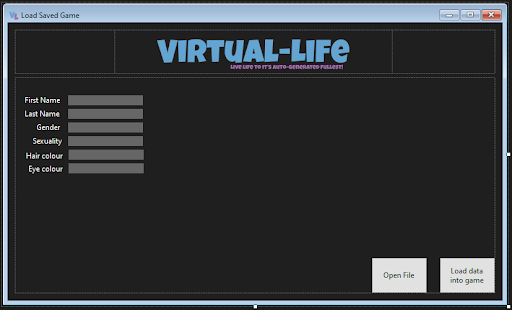
\includegraphics[width=0.8\textwidth]{images/implementation/showSavedGamesForm.png}
    \caption{Show saved games form}
    \label{fig:implementation-showSavedGamesForm}
\end{figure}

\section{File Handling}
One of the key elements of my success criteria was the ability to save a game to a file and read it back in when the app was opened again. \\
As I had worked with JSON files in previous projects before, I decided to use them for this project as I understood how to use them effectively. I did some research into saving to a JSON file and found a package called Newtonsoft. This package can serialize and deserialize the JSON file. The documentation for the package is bad at explaining why things work, so I spent quite a lot of time working out how to manually write the contents of each object out to an individual JSON file before I realised that part of the package might be able to do that for me. \newline
This is on my to-do list as a lower priority task as I feel like I'm focusing on the small details too much and not working on the actual game. I have also got a single object read back in by the program, however this is the only object in the file so I'm not sure if the same code will work when I introduce different objects to the file. At this moment in time, this isn\textquotesingle t meeting my success criteria.

\section{Loading Bar}
This wasn't in my design, however I believe it adds some value to the game, especially when handling files as wait times could be increased on slower systems.\\
It is a small form which appears with a marquee scrolling progress bar which says "Loading" on it, to tell the user that the game is doing something when the program is doing something; for example, when it is saving to a file.\\
The progress bar begins to move automatically, this is setup in the control properties within Visual Studio.
\begin{figure}[H]
    \centering
    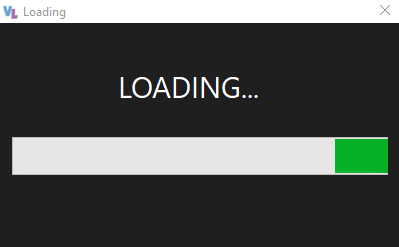
\includegraphics[width=0.4\textwidth]{images/implementation/loadingBarForm.png}
    \caption{Loading bar form}
    \label{fig:implementation-loadingBarForm}
\end{figure}

\begin{lstlisting}[language=c, style=csharp, caption=Code for the loadingbBar form]
public partial class frmLoadingBar : Form
{
    public frmLoadingBar()
    {
        InitializeComponent();
    }
}
\end{lstlisting}

\section{Building Main Game Screen form}
I began to build the form for the main game screen, by adding the TabControl which will allow me to have different tabs of information on one form, reducing the number of different forms which have to be loaded into memory at the same time; this also produces all-on-one-screen design which many of the games I played in research had.\\
After the TabControl, I added more panel controls to separate the different boxes of the information, to make resizing the form dynamically easier.
\begin{figure}[H]
    \centering
    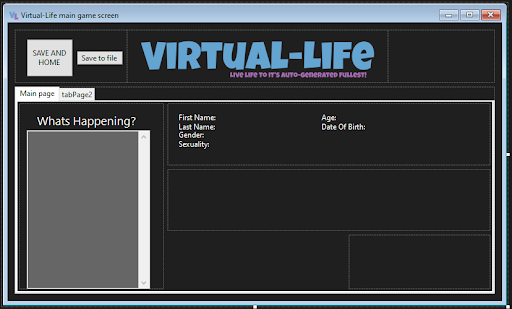
\includegraphics[width=0.8\textwidth]{images/implementation/buildingMainGameScreen.png}
    \caption{Work in progress of main game screen form}
    \label{fig:implementation-buildingMainGameScreen}
\end{figure}

\section{Array of Event Objects}
To store the various events I will have throughout the game, I will be creating an object for each one and to make programming and future maintenance easier, I will be storing them in an array.\\
I first wrote the code which made it work on one form. This worked the first time as I was following a tutorial and looking at errors which Visual Studio was giving me; correcting them as I programmed more. Then I setup the constructor for the next form in the game (main game screen) to receive the array of events object.
\begin{lstlisting}[language=c, style=csharp, caption=First attempt at declaring an array of objects]
Event[] eventArray = InitializeArray<Event>(numberOfEvents);
\end{lstlisting}
This resulted in the following error:\\
\verb|A field initializer cannot reference the non-static field, method, or property|\\ \verb|'frmNewGame.numberOfEvents'|\\
To fix this, I tried removing the variable numberOfEvents and changing it to a static integer like so:
\begin{lstlisting}[language=c, style=csharp, caption=Second attempt at declaring an array of objects]
Event[] eventArray = InitializeArray<Event>(10);
\end{lstlisting}
This still gave me the following error:\\
\verb|A field initializer cannot reference the non-static field, method, or property|\\ \verb|'frmNewGame.InitializeArray<Event>(int)'|\\
To try to fix this, I ignored the InitializeArray function and just declared a new array of objects:\\
\begin{lstlisting}[language=c, style=csharp, caption=Third attempt at declaring an array of objects]
public Event[] eventArray = new Event[10];
\end{lstlisting}
However, this gave me a null error saying the objects aren't defined.\\
I reverted back to the previous way and did some research - this pointed me at a Microsoft Docs page detailing Compiler Error CS0236.\\
From previous knowledge, I realised that compiler errors aren't something which are simple to understand, so I tried another option.\\
This gave me the following error:
\inlineCode{System.NullReferenceException:' Object reference not set to an instance of an object.' }\\
To resolve this error, I did more research and settled on the following solution.\\
This first block of code comes from when the new game screen form is loaded.
\begin{lstlisting}[language=c, style=csharp, caption=Final solution for declaring an array of objects part 1]
//Create array of event object called eventArray
public int numberOfEvents = 1000;
public Event[] eventArray = new Event[1000];
public int nextEvent = 0;
\end{lstlisting}
This next block of code is run when the save button is pressed
\begin{lstlisting}[language=c, style=csharp, caption=Final solution for declaring an array of objects part 2]
//create event objects needed for game
for (int i = 0; i < controlClass.NumberOfEvents; i++)
{
    eventArray[i] = new Event();
}
\end{lstlisting}
This works by setting up the integer variable \verb|numberOfEvents| then the array of type \verb|Event| containing 1000 \verb|Event| objects and then the integer variable \verb|nextEvent| which would be used to find the next available slot in the array meaning I could very quickly input the next item in the array without having to locate it every time I needed to enter something into it. The \verb|numberOfEvents| variable could be set dynamically using an inbuilt C\# method for array handling - my intention is to change this over. This change would mean that I would only need to change the length of the array once in the program and the change would be reflected all throughout the code.
After I had added the code which is needed to populate the array:
\begin{lstlisting}[language=c, style=csharp, caption=Code needed to create the first event in the array]
eventArray[controlClass.NextEvent].Category = "Life Event";
eventArray[controlClass.NextEvent].DateHappened = DateTime.Today;
eventArray[controlClass.NextEvent].Description = "You were born to parents xxx;
controlClass.NextEvent++;
\end{lstlisting}
I tested it and I got the outcome which I wanted to see - the text box on the main game screen showing the event.
\begin{figure}[H]
    \centering
    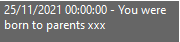
\includegraphics[width=0.4\textwidth]{images/implementation/eventArrayDemo.png}
    \caption{Evidence that the array of Event objects are being constructed correctly}
    \label{fig:implementation-eventArrayDemo}
\end{figure}

\section{File Handling - Attempt 2}
When I worked on loading the saved files into the game, I realised that the JSON package handler I was using had a serialisation and deserialization function built in which is much more elegant and resource efficient than the method which I was using. I looked into the different methods which came with \verb|Newtonsoft.Json| and found the \verb|JsonConvert.SerializeObject(objectName)| and tested writing out to a file using that. This worked first time with the following code.
\begin{lstlisting}[language=c, style=csharp, caption=Code used to write out to JSON files]
File.WriteAllText(filepath, JsonConvert.SerializeObject(mainCharacter));
\end{lstlisting}
However, I also had to include \verb|Newtonsoft.Json| separately to \verb|Newtonsoft.Json.Linq| at the top of the project. I then began to look at how to write out the other objects to the file.
It was extremely difficult to get the writing out and reading in working. I spent a lot of time following tutorials which ended in an error or not the result I was expecting. I decided that to make this work, I would need to go back to basics and work out exactly what I needed, not what I wanted. This re-designing allowed me to realise that there was no need for all the objects to be written out to the same file, they could be in fact written out to separate files within one folder. This epiphany resulted in me solving how to get the objects written out to separate files, and read them in again. To write them out, I did it in much the same way as before however, in my \verb|File.WriteAllText| statement, I also had to include the file name. The code below shows how a single object is written out to a JSON file. This is repeated multiple times in the code with the filepath and object name substituted.
\begin{lstlisting}[language=c, style=csharp, caption=Code used to write out to JSON files]
File.WriteAllText(controlClass.Filepath + "\\mainCharacter.json", JsonConvert.SerializeObject(mainCharacter));
\end{lstlisting}
This was much the same for when a file is being opened.
\begin{lstlisting}[language=c, style=csharp, caption=Code used to open a JSON file and read the contents of it into an object]
MainCharacter mainCharacter = JsonConvert.DeserializeObject<MainCharacter>(File.ReadAllText(loadFilepath + "\\mainCharacter.json"));
\end{lstlisting}
To select the folder which I was going to be using, I used a FolderBrowserDialog control which comes as standard with the Windows Form Library.

\section{Control Class}
Whilst designing the file management system, I realised that there were lots of data items which would need to be stored alongside the game for the game to work. Up until now, I had been storing them as variables but hadn't thought about how I would need to save them. I decided to save them as an object, this way I can easily save to a file in the same way I am doing for the other objects.
This control class also means I am able to pass data between forms much simpler, as I can simply pass the entirety of the \verb|controlClass| to the new form rather than the individual attributes separately.
\begin{lstlisting}[language=c, style=csharp, caption=Declaration of Control Class]
public class ControlClass
{
    //private attributes
    private DateTime inGameDate;
    private int numberOfEvents;
    private int nextEvent;
    private string filepath;
    private int numberOfFamily;
    private int nextFamily;
    private string nameOfCurrentSchool;
    private int currentSchoolYear;
    private int eduScorePlus;
    private int happinessScorePlus;


    //get and sets
    //GENERIC GAME STUFF----
    public DateTime InGameDate { get; set; }
    public string Filepath { get; set; }
    //EVENTS-------
    public int NumberOfEvents { get; set; }
    public int NextEvent { get; set; }
    //FAMILY--------
    public int NumberOfFamily { get; set; }
    public int NextFamily { get; set; }
    //EDUCATION------
    public string NameOfCurrentSchool { get; set; }
    public int CurrentSchoolYear { get; set; }
    public int EduScorePlus { get; set; }

    //HAPPINESS SCORE-----
    public int HappinessScorePlus { get; set; }

}
\end{lstlisting}

\section{Random Generation of Family Members}
I decided that I would be using the constructor of the \verb|GenericFamilyMember| class to populate the attributes of each object. To differentiate between each family member, I will be passing into the constructor the number in the \verb|familyArray|, allowing me to use a switch statement to differentiate between family members.\\
To start with, I am using 2 attributes of index 0, which is the father of the main character. This will allow me to test the random generation aspect (in the \verb|FirstName| attribute) and the fixed value aspect (in the \verb|RelationshipToMain| attribute).\\
I wrote the following code.

\begin{lstlisting}[language=c, style=csharp, caption=Initial test of generating a Random Character]
public GenericFamilyMember(int charNumber)
{
    //construct here
    //go through a switch statement to set the character based on what their relationship to the main is.
    switch(charNumber)
    {
        case 0:
            //Dad to main character
            FirstName = genMFN();
            RelationshipToMain = "Father";
            break;
        default:
            FirstName = null;
            break;
    }
}

//Generate a Male first name
public static string genMFN()
{
    //generate male first name
    string[] name = { "Liam", "Noah", "Oliver", "Elijah", "William", "James", "Benjamin", "Ben", "Lucas", "Henry", "Alex", "Ethan", "Daniel", "Sebstian", "Jack", "Matt", "John", "Joe", "David", "Josh", "Julien", "Leo", "Isaac", "Thomas", "Max", "Andy", "Phill", "Harvey", "Ryan" };
    string returnName = name[rnd.Next(1, 29)];
    return returnName;
}
\end{lstlisting}
This produced the following error: \inlineCode{CS0120 An object reference is required for the non-static field, method or property 'GenericFamilymember.rnd'}\\
To solve this, I moved the constructor for the \verb|Random| class to the function \verb|genMFN|. This worked, and allowed me to generate a random number which I then used to select one of the names in the array name.
\begin{lstlisting}[language=c, style=csharp, caption=Creating a Random object of class Random for later use]
Random rnd = new Random();
\end{lstlisting}
The data now appeared as I was expecting it to do in the \verb|familyArray| file.
\begin{figure}[H]
    \centering
    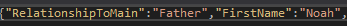
\includegraphics[width=0.8\textwidth]{images/implementation/familyArrayData.png}
    \caption{Screenshot of familyArray file containing correct data}
    \label{fig:implementation-familyArrayData}
\end{figure}
\noindent As I was creating more of the constructor methods, I realised that it would make more sense to move the random generation functions into the \verb|Person| class so that all of the subclasses can use them for their own character generation. The code now looks like this
\begin{lstlisting}[language=c, style=csharp, caption=Random name generation functions]
 //functions used in constructors
public static string genLN()
{
    //Generate female first name
    Random rnd = new Random();
    string[] name = { "Smith", "Brown", "Wilson", "Thomson", "Robertson", "Campbell", "Stewart", "Macdonald", "Murray", "Reid", "Taylor", "Clark", "Mitchell", "Ross", "Watson", "Miller", "Gray", "Simpson", "Duncan", "Bell", "Grant", "Mackenzie", "Allan", "Wood", "Muir", "Watt", "King", "Bruce", "Boyle", "Douglas" };
    string returnName = name[rnd.Next(1, 29)];
    return returnName;
}
public static string genMFN()
{
    //generate male first name
    Random rnd = new Random();
    string[] name = { "Liam", "Noah", "Oliver", "Elijah", "William", "James", "Benjamin", "Ben", "Lucas", "Henry", "Alex", "Ethan", "Daniel", "Sebstian", "Jack", "Matt", "John", "Joe", "David", "Josh", "Julien", "Leo", "Isaac", "Thomas", "Max", "Andy", "Phill", "Harvey", "Ryan" };
    string returnName = name[rnd.Next(1, 29)];
    return returnName;
}

public static string genFFN()
{
    //Generate female first name
    Random rnd = new Random();
    string[] name = { "Olivia", "Sophia", "Maria", "Mia", "Evelyn", "Jess", "Ella", "Zoe", "Jemma", "Gemma", "Emily", "Nuala", "Maggie", "Ciara", "Scarlett", "Layla", "Chloe", "Ellie", "Hazel", "Lucy", "Niamh", "Kat", "Victoria", "Lily", "Hannah", "Chloe", "Lara", "Bella", "Ruby" };
    string returnName = name[rnd.Next(1, 29)];
    return returnName;
}
\end{lstlisting}
I then tested opening a saved game and got an error as the JSON deserialize function creates new instances of the \verb|GenericFamilyMember| to populate as it reads in the file. To fix this, I moved the constructor into a separate method within the \verb|GenericFamilyMember| class and called it like this (shown from the new game form)
\begin{lstlisting}[language=c, style=csharp, caption=Code used to generate generic family members]
for (int i = 0; i < controlClass.NumberOfFamily; i++)
{
    GenericFamilyMember tempFamily = new GenericFamilyMember(); //make new instance of the object
    tempFamily.populateGenericFamilyMember(i, mainCharacter); //populate that object using the 'constructor' in the GenericFamilyMemberclass
    familyArray[i] = tempFamily; //transfer the temp object into the array.
}
\end{lstlisting}

\noindent I then moved onto the generation of the date of birth. To do this, I wrote the following function, which produces a date between 16 and 30 years ago. 
\begin{lstlisting}[language=c, style=csharp, caption=Function which generates DoB of parent]
static DateTime genParentAge(DateTime mcDOB)
{
    //need to generate a date between 16 and 30 years ago from main character birthday.
    DateTime dateOfBirth;
    Random rand = new Random();
    int randomNumber = rand.Next(5845, 10957);
    dateOfBirth = mcDOB.AddDays(-randomNumber);


    return dateOfBirth;
}
\end{lstlisting}
When I tested it, I got the following result; proving it works.
\begin{figure}[H]
    \centering
    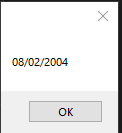
\includegraphics[width=0.3\textwidth]{images/implementation/proofParentAgeGenWorks.png}
    \caption{Proof that the parent DoB generation algorithm works}
    \label{fig:implementation-proofParentAgeGenWorks}
\end{figure}
\noindent As this is working for the father, I implemented it for the mother as well.\\
I then implemented the age calculation algorithm, I thought about a number of different ways I could do this and settled on passing in the character's birthday and returning an integer containing their age.
\begin{lstlisting}[language=c, style=csharp, caption=Age generation algorithm]
public int calcAge(DateTime input)
{
    int difference = (DateTime.Today.Date - input.Date).Days;
    float toround = (difference / 365);
    int age = ((int)toround);

    return age;
}
\end{lstlisting}
This worked first time so I implemented it for the mother as well.\\
The age was the last element I had to programmatically generate for the main character's parents. The finished constructor for the mum and dad can be seen below:
\begin{lstlisting}[language=c, style=csharp, caption=Final code for generation of mother and father to main character]
public GenericFamilyMember populateGenericFamilyMember(int charNumber, MainCharacter mainCharacter)
{
    //construct here
    //go through a swtich statement to set the character based on what their relationship to the main is.
    //setup random number generation
    Random rnd = new Random();
    GenericFamilyMember familyMember = new GenericFamilyMember();
    switch (charNumber)
    {
        case 0:
            //Dad to main character
            RelationshipToMain = "Father";
            FirstName = genMFN();
            LastName = mainCharacter.LastName;
            Gender = "Male";
            Sexuality = "Straight";
            DateOfBirth = genParentAge(mainCharacter.DateOfBirth);
            LivingStatus = true;
            InRelationship = true;
            Age = calcAge(DateOfBirth);
            break;
        case 1:
            //mum to main character
            RelationshipToMain = "Mother";
            FirstName = genFFN();
            switch (rnd.Next(1, 3))
            {
                case 1:
                    //same last name as father and main character
                    LastName = mainCharacter.LastName;
                    break;
                case 2:
                default:
                    //different last name to father and main character - need to randomGen this
                    LastName = genLN();
                    break;
            }
            Gender = "Female";
            Sexuality = "Straight";
            DateOfBirth = genParentAge(mainCharacter.DateOfBirth);
            LivingStatus = true;
            InRelationship = true;
            Age = calcAge(DateOfBirth);
            break;
        default:
            FirstName = null;
            break;
    }
    return familyMember;
}
\end{lstlisting}
While generating a new family member, I received an index out of bounds error for the random name generation. To fix this, I change the top random number to 30 as I had forgotten that arrays are zero-based therefore they don't actually have an item 30 therefore the random generation top bound would need to be reduced by 1. I also moved the random generation lower bound down to 0, to accommodate for the zero-based nature of the array.

\section{Family Tab}
Now I have developed the generation of the various characters, I need a way to display them. I am using the \verb|DataGridView| control which presents the data in table. I did some research and found the following line of code which works and displays the following.
\begin{lstlisting}[language=c, style=csharp, caption=First attempt at using a DataGridView control to show the family tab.]
dgvFamily.DataSource = familyArray;
\end{lstlisting}
\begin{figure}[H]
    \centering
    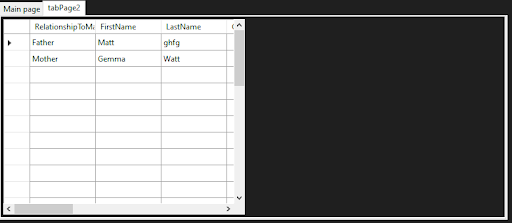
\includegraphics[width=0.8\textwidth]{images/implementation/familyTabInitialTest.png}
    \caption{Result of initial test of using the DataGridView control for the family tab.}
    \label{fig:implementation-familyTabInitialTest}
\end{figure}
\noindent This displays the whole object at once - meaning the user has to scroll horizontally to see all the data. This is not what I wanted so I went back through my old projects and found the code that did what I wanted.
\begin{lstlisting}[language=c, style=csharp, caption=Improved method of populating dgvFamily]
 //first, set var for which column contains which data
int relationshipCol = 0;
int firstNameCol = 1;
int lastNameCol = 2;

//now loop through familyArray and populate dgvFamily
// can use a for loop as number of family members are in the controlClass

for(int x=0; x<controlClass.NumberOfFamily; x++)
{
    int i = dgvFamily.Rows.Add();
    dgvFamily.Rows[i].Cells[relationshipCol].Value = familyArray[x].RelationshipToMain;
    dgvFamily.Rows[i].Cells[firstNameCol].Value = familyArray[x].FirstName;
    dgvFamily.Rows[i].Cells[lastNameCol].Value = familyArray[x].LastName;
}
\end{lstlisting}
This gave me an error: \inlineCode{System.InvalidOperationException: 'Rows cannot be programmatically added to the DataGridView's rows collection when the control is data-bound.'}\\
Which I rectified by removing the previous line of code used by commenting it out. This worked and gave me the result I expected. (At this point, I had also added some colors to the control using Visual Studio's property panel).
\begin{figure}[H]
    \centering
    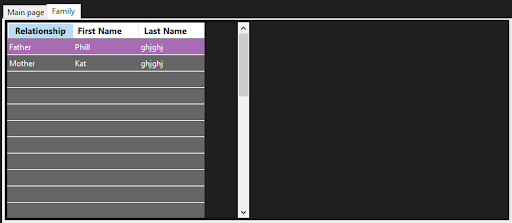
\includegraphics[width=0.8\textwidth]{images/implementation/familyTabSecondTest.png}
    \caption{Second test of displaying information on the DataGridView control}
    \label{fig:implementation-familyTabSecondTest}
\end{figure}
\noindent Now I have the basic code working, I want to change it so it only shows the entries in the array which have data in them. I will do this by including an IF statement inside the FOR loop, like so:
\begin{lstlisting}[language=c, style=csharp, caption=Improved code for displaying data in the DataGridView]
for(int x=0; x<controlClass.NumberOfFamily; x++)
{
    if (familyArray[x].FirstName != null)
    {
        int i = dgvFamily.Rows.Add();
        dgvFamily.Rows[i].Cells[relationshipCol].Value = familyArray[x].RelationshipToMain;
        dgvFamily.Rows[i].Cells[firstNameCol].Value = familyArray[x].FirstName;
        dgvFamily.Rows[i].Cells[lastNameCol].Value = familyArray[x].LastName;
    }
}
\end{lstlisting}
This works and the DataGridView now looks like this:
\begin{figure}[H]
    \centering
    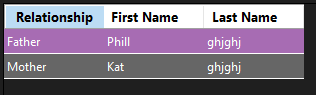
\includegraphics[width=0.4\textwidth]{images/implementation/familyTabFinalDGVTest.png}
    \caption{The DataGridView showing populated rows only}
    \label{fig:implementation-familyTabFinalDGVTest}
\end{figure}
\noindent I then added the code which populates the label controls on the form - this allows the person's information to be displayed to the player.
\begin{lstlisting}[language=c, style=csharp, caption=Code to populate labels on Family Tab containing information about the selected person]
private void dgvFamily_CellContentClick(object sender, DataGridViewCellEventArgs e)
{
   // MessageBox.Show(dgvFamily.CurrentCell.RowIndex.ToString());
    int currentIndex = dgvFamily.CurrentCell.RowIndex;
    //MessageBox.Show(familyArray[currentIndex].Age.ToString());

    //populate info on form
    lblFamRealtionshipToMain.Text = mainCharacter.FirstName + "'s " + familyArray[currentIndex].RelationshipToMain;
    lblFamFirstName.Text = "First Name: " + familyArray[currentIndex].FirstName;
    lblFamLastName.Text = "Last Name: " + familyArray[currentIndex].LastName;
    lblFamGender.Text = "Gender: " + familyArray[currentIndex].Gender;
    lblFamSexuality.Text = "Sexuality: " + familyArray[currentIndex].Sexuality;
    lblFamAge.Text = "Age: " + familyArray[currentIndex].Age.ToString();
    lblFamLivingStatus.Text = "Living Status: " + familyArray[currentIndex].LivingStatus.ToString();
    lblFamDateOfBirth.Text = "Date Of Birth: " + familyArray[currentIndex].DateOfBirth.ToShortDateString();
    lblFamInRelationship.Text = "In Relationship: " + familyArray[currentIndex].InRelationship.ToString();
    if(familyArray[currentIndex].LivingStatus == false)
    {
        //person is dead so can show death date and reason for death
        lblFamDateOfDeath.Text = "Date Of Death: " + familyArray[currentIndex].DateOfDeath.ToShortDateString();
        lblFamReasonForDeath.Text = "Reason For Death: " + familyArray[currentIndex].ReasonForDeath;
    }
    else
    {
        //person is not dead - don't show death date and reason for death
        lblFamDateOfDeath.Text = "Date Of Death: N/A (haven't died yet!)";
        lblFamReasonForDeath.Text = "Reason For Death: N/A (haven't died yet!)";
    }
}
\end{lstlisting}
\begin{figure}[H]
    \centering
    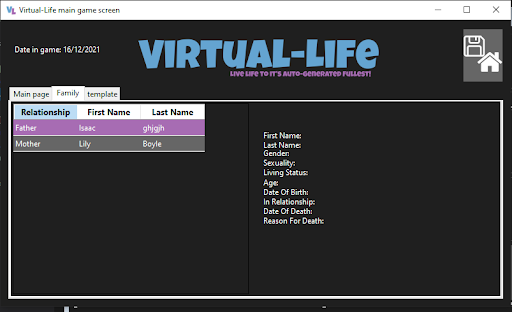
\includegraphics[width=0.8\textwidth]{images/implementation/familyTabLabelsPre.png}
    \caption{Empty labels, before any information is put into them}
    \label{fig:implementation-familyTabLabelsPre}
\end{figure}
\begin{figure}[H]
    \centering
    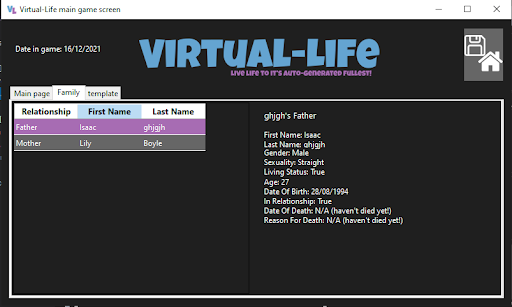
\includegraphics[width=0.8\textwidth]{images/implementation/familyTabLabelsPost.png}
    \caption{Filled out labels, after the father has been selected}
    \label{fig:implementation-familyTabLabelsPost}
\end{figure}
\noindent In the figures above, it looks like the father has been selected before it actually has. This is a feature of the \verb|DataGridView|, in that there has to be a row \textquotesingle selected\textquotesingle  at all times.

\section{Loading the Files in}
During developmental testing, I realised that I had quite a serious bug. From moving from system to system, the filepath of the game wasn't dynamically adapting to the system, meaning I couldn't use a save I made on the college computer at home as the file path in the control class was wrong. To resolve this issue, I added this line of code to the opening files form:
\begin{lstlisting}[language=c, style=csharp, caption=Line of code used to fix the filepath issues]
controlClass.Filepath = filepath;
\end{lstlisting}
This overrides whatever had been read in from the control class file with the location specified by the user to find the saved data from the game.

\section{Death}
Now, I need to start processing the events of the age up algorithm, the first thing I am going to program is the death checker. This algorithm will check based on the character\textquotesingle s age the probability of them dying and return a boolean for if they shall live or not, if they don't live, then their data will be sent to another subroutine which will ‘kill' them and update the relevant variables to reflect this. I started by testing the ageing up of family members and realised that I hadn't yet programmed this. This means I have to do this first.\\
I added a procedure in which loops through all the elements of the array \verb|familyArray| and if the living status is true, then it adds 1 to the age of the character. This will allow me to not age up characters once they have died.
\begin{lstlisting}[language=c, style=csharp, caption=Method which increases the age of the family array]
private void ageUpFamilyArray()
{
    //loop through all the members of the family array and add 1 to their age if livingstatus is true
    for(int x=0; x<controlClass.NumberOfFamily; x++)
    {
        if(familyArray[x].LivingStatus == true)
        {
            //can age them up
            familyArray[x].Age = familyArray[x].Age + 1;
        }
    }
}
\end{lstlisting}
To confirm that this was working as intended, I ran the code and confirmed the father of the main characters age before and after I pressed the age up button. It behaved as expected; therefore I was satisfied to move onto the next aspect of the death checker.\\
I added the following code which changes the chance of the main character dying based on their age.
\begin{lstlisting}[language=c, style=csharp, caption=Main character death checker algorithm]
public bool deathCheckerMainCharacter(int age)
{
    bool deathBool = false;
    
    int age = mainCharacter.Age;
    int deathChance = 1;
    //for as main char gets older, their death chance increases
    /* 00-10 1/30 
     * 11-16 1/25
     * 17-30 1/15 
     * 31-50 1/25 
     * 51-67 1/20 
     * 68-80 1/15 
     * 81-100 1/8 
     * >100 1/3 
     */
    if (age <= 10)
    {
        deathChance = 30;
    }
    else if (age >= 11 && age <= 16)
    {
        deathChance = 25;
    }
    else if (age >= 17 && age <= 30)
    {
        deathChance = 15;
    }
    else if (age >= 31 && age <= 50)
    {
        deathChance = 25;
    }
    else if (age >= 51 && age <= 67)
    {
        deathChance = 20;
    }
    else if (age >= 68 && age <= 80)
    {
        deathChance = 15;
    }
    else if (age >= 81 && age <= 99)
    {
        deathChance = 8;
    }
    else if (age >= 100)
    {
        deathChance = 3;
    }
    //now generate random number based off of 1 and deathChance
    Random rnd = new Random();
    int randomReturn = rnd.Next(1, deathChance);
    if (randomReturn == 2)
    {
        //DEATH
        deathBool = true;
    }
    else
    {
        deathBool = false;
    }

    //return deathBool to main program where it will be processed.
    return deathBool;
}
\end{lstlisting}
I then added the code which will programmatically kill the main character:
\begin{lstlisting}[language=c, style=csharp, caption=Kill main character method]
public void killMainCharacter()
{
    //very rough for now, will need to polish at some point

    btnAgeUp.Enabled = false;
    mainCharacter.DateOfDeath = controlClass.InGameDate; 
    mainCharacter.LivingStatus = false;
    mainCharacter.ReasonForDeath = generateReasonForDeath();
    //generate event showing this
    eventArray[controlClass.NextEvent].Category = "Death";
    eventArray[controlClass.NextEvent].DateHappened = controlClass.InGameDate;
    eventArray[controlClass.NextEvent].Description = "You died due to " + mainCharacter.ReasonForDeath;
    controlClass.NextEvent++;
    MessageBox.Show(mainCharacter.FirstName + " has died a tragic death due to " + mainCharacter.ReasonForDeath, mainCharacter.FirstName + " has died", MessageBoxButtons.OK, MessageBoxIcon.Exclamation);
    saveToFile();
}
\end{lstlisting}
This produces the outcome of:
\begin{figure}[H]
    \centering
    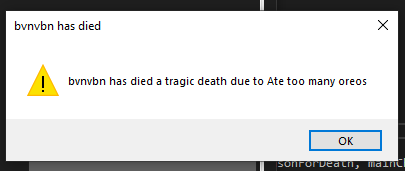
\includegraphics[width=0.5\textwidth]{images/implementation/deathProof1.png}
    \caption{Alerting message box displayed when Main Character Dies}
    \label{fig:implementation-deathProof1}
\end{figure}
\begin{figure}[H]
    \centering
    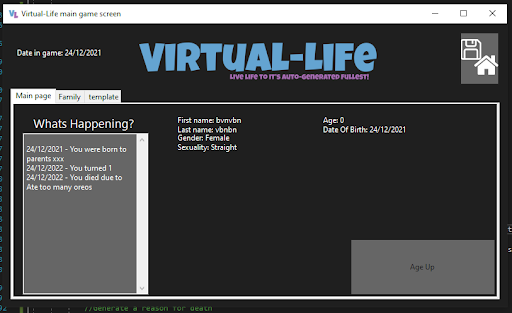
\includegraphics[width=0.8\textwidth]{images/implementation/deathProof2.png}
    \caption{Main game screen showing death event and age up button disabled}
    \label{fig:implementation-deathProof2}
\end{figure}
\noindent I then moved onto the killing algorithm of the other characters, this will be done in a similar way to the increasing age of them - looping through the array and if they aren't already dead then passing them through the death checker then if they are to die, passing them through a kill procedure which will make use of the same \verb|generateReasonForDeath| function.
This was very easy to program as I had already worked out the fundamentals of this in the main character killing functions, so I was able to copy, paste and adapt the code to suit the \verb|genericFamilyMember| objects.
\begin{lstlisting}[language=c, style=csharp, caption=Death algorithm for a non-main character]
public void checkKillGenericFamilyMember()
{
    //loop through all members of familyArray, passing their age into deathCheck. if return=true then kill, else move onto next.

    for(int x=0; x<controlClass.NextFamily; x++)
    {
        if(familyArray[x].LivingStatus == true)
        {
            bool deathCheckReturn = deathCheck(familyArray[x].Age);
            if(deathCheckReturn == true)
            {
                //RIP - put death code here
                //MessageBox.Show("DEATH" + x.ToString());
                familyArray[x].DateOfDeath = controlClass.InGameDate.AddDays(randomNumber(1, 300));
                familyArray[x].LivingStatus = false;
                familyArray[x].ReasonForDeath = generateReasonForDeath();
                //Now gen event
                eventArray[controlClass.NextEvent].Category = "Death";
                eventArray[controlClass.NextEvent].DateHappened = controlClass.InGameDate;
                eventArray[controlClass.NextEvent].Description = familyArray[x].FirstName + " (your " + familyArray[x].RelationshipToMain.ToLower() + ") died due to " + familyArray[x].ReasonForDeath;
                controlClass.NextEvent++;
                //now reduce mc happiness score
                mainCharacterScores.HappinessScore = mainCharacterScores.HappinessScore - randomNumber(1, 100);
                saveToFile();
            }
        }
    }
}
\end{lstlisting}
For the purposes of testing, I added in a line of code which will force the character to die. This is omitted from the code above.\\
\begin{figure}[H]
    \centering
    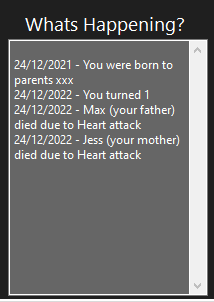
\includegraphics[width=0.3\textwidth]{images/implementation/deathProofGeneric.png}
    \caption{Event box on main game screen showing someone has died}
    \label{fig:implementation-deathProofGeneric}
\end{figure}
I then included more reasons for death. My reasons for death array now contains the following:
\begin{lstlisting}[language=c, style=csharp, caption=Reasons for death array]
string[] reasonsForDeath = { "a heart attack", "eating too many oreos", "being clawed at by cat" , "slipping on a banana peel", "falling in the otter enclosure at a zoo and being licked to death", "dropping a toaster into the bath", "being crushed by a falling grand piano", "being strangled by a fez tassel", "walking into a cactus", "getting hit by a train", "being clubbed by old lady in the street with her walker", "being crushed by a stampede of hungry campers"};
\end{lstlisting}

\section{Random Generation Of a Main Character}
At this point in developmental testing, I was creating a new game relatively frequently, to allow me to test different aspects. It takes about a minute to setup the main character in the new game form, even with just entering gobbledygook. To improve on this time, I created a random generation button with the following code behind it.
\begin{lstlisting}[language=c, style=csharp, caption=Random generation of main character algorithm]
private void btnRandom_Click(object sender, EventArgs e)
{
    Random rnd = new Random();
    int gender = rnd.Next(1, 3);
    switch (gender)
    {
        case 1:
            //male
            txtFirstName.Text = Person.genMFN();
            cboGender.Text = "Male";
            break;
        case 2:
            //female
            txtFirstName.Text = Person.genFFN();
            cboGender.Text = "Female";
            break;
        default:
            txtFirstName.Text = "Sam";
            break;
    }
    txtLastName.Text = Person.genLN();
    int hair = rnd.Next(1,5);
    int eye = rnd.Next(1, 6);

    switch (hair)
    {
        case 1:
            cboHairColour.Text = "Blonde";
            break;
        case 2:
            cboHairColour.Text = "Brown";
            break;
        case 3:
            cboHairColour.Text = "Red";
            break;
        case 4:
            cboHairColour.Text = "Black";
            break;
        default:
            cboHairColour.Text = "Blonde";
            break;
    }

    switch (eye)
    {
        case 1:
            cboEyeColour.Text = "Brown";
            break;
        case 2:
            cboEyeColour.Text = "Blue";
            break;
        case 3:
            cboEyeColour.Text = "Green";
            break;
        case 4:
            cboEyeColour.Text = "Gray";
            break;
        case 5:
            cboEyeColour.Text = "Amber";
            break;
        default:
            cboEyeColour.Text = "Brown";
            break;
    }
    
}
\end{lstlisting}
This works as expected and produces a random character.

\section{Scores}
Before I programmed any more of the game, I decided that I would need to add in the code for my scores. I first added the \verb|Score| class.
\begin{lstlisting}[language=c, style=csharp, caption=Score class]
public class Score
{
    private int educationScore;
    private int jobScore;
    private int happinessScore;
    private int medicalScore;
    private int lifeScore;

    public int EducationScore { get; set; }
    public int JobScore { get; set; }
    public int HappinessScore { get; set; }
    public int MedicalScore { get; set; }
    public int LifeScore { get; set; }
}
\end{lstlisting}
I then added the code to the constructor of the create new game form which will create a new object called \verb|mainCharacterScores|.
\begin{lstlisting}[language=c, style=csharp, caption=Declaration of the mainCharacterScores object]
public Score mainCharacterScores = new Score();
\end{lstlisting}
I then added the the initialisation code with placeholder values.
\begin{lstlisting}[language=c, style=csharp, caption=Setting the score values to placeholder values]
//setup the scores object for the main (use random generation to calculate values)
mainCharacterScores.EducationScore = 0;
mainCharacterScores.JobScore = 0;
mainCharacterScores.HappinessScore = 0;
mainCharacterScores.MedicalScore = 0;
mainCharacterScores.LifeScore = 0;
\end{lstlisting}
Now, I need to add the code to write this new object out to a file (on the \verb|MainGameScreen| form)
\begin{lstlisting}[language=c, style=csharp, caption=Code to write the Scores object out to a file]
File.WriteAllText(controlClass.Filepath + "\\mainCharacterScores.json", JsonConvert.SerializeObject(mainCharacterScores));
\end{lstlisting}
To test this first, I created a new game then saved it and viewed the \verb|mainCharacterScores.Json| file in Notepad++. I saw what I was expecting
\begin{figure}[H]
    \centering
    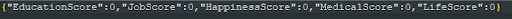
\includegraphics[width=0.8\textwidth]{images/implementation/scoresTest1.png}
    \caption{Screenshot of Notepad++ showing scores object}
    \label{fig:implementation-scoresTest1}
\end{figure}
\noindent Now I can write the data out to a file, I need a way to read it back into the game. I added the code needed in the show saved games form for this.
\begin{lstlisting}[language=c, style=csharp, caption=Code to read mainCharacterScores back in]
Score mainCharacterScores = JsonConvert.DeserializeObject<Score>(File.ReadAllText(filepath + "\\mainCharacterScores.json"));
\end{lstlisting}
I then added the code in to show the life score in a message box, so I could test opening the same saved game files.
\begin{lstlisting}[language=c, style=csharp, caption=Test code to make sure code above is working]
MessageBox.Show(mainCharacterScores.LifeScore.ToString());
\end{lstlisting}
This worked as expected and produced the following result
\begin{figure}[H]
    \centering
    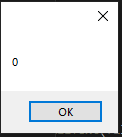
\includegraphics[width=0.2\textwidth]{images/implementation/scoresTest2.png}
    \caption{Proof the scores are being read back into the program correctly}
    \label{fig:implementation-scoresTest2}
\end{figure}
\noindent I then removed the code for the message box because now that I know that the file management is working, I can now add in the algorithms for all these values and the displays in the game window for them. To start, I will add in the code to the create new game form to randomly generate the initial score values. I will be using an instance of the \verb|Random| class called \verb|rnd| to generate the scores. Each score will have a maximum value of 100.
\begin{lstlisting}[language=c, style=csharp, caption=Setting the score values random values]
//setup the scores object for the main (use random generation to calculate values)
mainCharacterScores.EducationScore = rnd.Next(0, 101);
mainCharacterScores.JobScore = rnd.Next(0, 101);
mainCharacterScores.HappinessScore = rnd.Next(0, 101);
mainCharacterScores.MedicalScore = rnd.Next(0, 101);
mainCharacterScores.LifeScore = rnd.Next(0, 101);
\end{lstlisting}
To display this information, I will take inspiration from one of the games which I was playing during research - using a bar to represent the information. I will use the control ProgressBar as they are easy to set the value of and a nice visual representation of the value.
\begin{figure}[H]
    \centering
    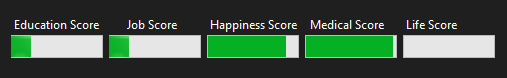
\includegraphics[width=0.8\textwidth]{images/implementation/scoresTest3.png}
    \caption{Progress bar controls containing the score values}
    \label{fig:implementation-scoresTest3}
\end{figure}
\noindent (Colours and placement are subject to redesign)\\
I then added the code to make each of the progress bars fill depending on the value of the score.
\begin{lstlisting}[language=c, style=csharp, caption=Code to display the score in the progress bar]
public void updateScoresPB()
{
    prbEducationScore.Value = mainCharacterScores.EducationScore;
    prbJobScore.Value = mainCharacterScores.JobScore;
    prbHappinessScore.Value = mainCharacterScores.HappinessScore;
    prbMedicalScore.Value = mainCharacterScores.MedicalScore;
    prbLifeScore.Value = mainCharacterScores.LifeScore;
}
\end{lstlisting}
As with most of my program, I am breaking it down into smaller functions or procedures as I will need to use the code in many different places.

\section{Education}
Now I have my scores and displaying of said scores working, I can begin writing the code which will alter the scores. The first score I will program is the education score. To start off, I setup the code which will calculate the next 1st September based off of the character's date of birth then work out what year they should be moving into in school.
\begin{lstlisting}[language=c, style=csharp, caption=Procedure to check the education status of the main character]
public void checkEducationStatus()
{
    int age = mainCharacter.Age;
    DateTime mcBirthday = mainCharacter.DateOfBirth;
    DateTime dateOfEvent;
    if (mcBirthday.DayOfYear < 245)
    {
        //mc is born before 2nd sept therefor events need to be for this september
        int yearOfEvent = controlClass.InGameDate.Year;
        int monthOfEvent = 9;
        int dayOfEvent = 1;
        dateOfEvent = new DateTime(yearOfEvent, monthOfEvent, dayOfEvent);
    }
    else
    {
        //mc is born after 2nd sept therfore events need to be for the following september
        int yearOfEvent = (controlClass.InGameDate.Year) + 1;
        int monthOfEvent = 9;
        int dayOfEvent = 1;
        dateOfEvent = new DateTime(yearOfEvent, monthOfEvent, dayOfEvent);
    }
    //need to get date of 1st september after mcs birthday
    switch (age)
    {
        case 4:
            //move into reception
            eventArray[controlClass.NextEvent].Category = "Education";
            eventArray[controlClass.NextEvent].DateHappened = dateOfEvent;
            eventArray[controlClass.NextEvent].Description = "Move into year 4";
            controlClass.NextEvent++;
            break;
\end{lstlisting}
For testing, I have just used the first year - age 4 where the character will be entering reception. The test code I wrote works and displays the following. Where it says  'move into year4', this should read 'move into reception'. This is not an program error, this is a typing error on my part.
\begin{figure}[H]
    \centering
    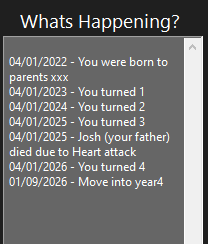
\includegraphics[width=0.3\textwidth]{images/implementation/educationTest1.png}
    \caption{Event box showing first school event}
    \label{fig:implementation-educationTest1}
\end{figure}
\noindent I then setup the page of the TabControl which will display the education information. It is basic for the moment, this may be improved at a later point.
\begin{figure}[H]
    \centering
    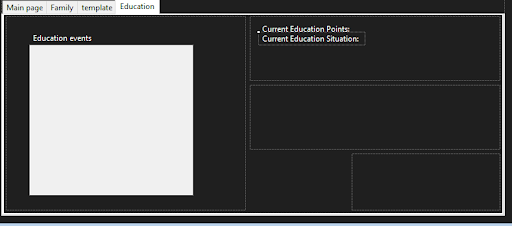
\includegraphics[width=0.8\textwidth]{images/implementation/educationTest2.png}
    \caption{TabControl showing education page}
    \label{fig:implementation-educationTest2}
\end{figure}
\noindent Now, I will add the code to populate the form.
\begin{lstlisting}[language=c, style=csharp, caption=Code to populate the education page on the main game form]
public void updateEducationPage()
{
    //first update the events box
    txtEduEducationEvents.ResetText();
    for (int i = 0; i < controlClass.NextEvent; i++)
    {
        if(eventArray[i].Category == "Education")
        {
            txtEduEducationEvents.Text = txtEduEducationEvents.Text + Environment.NewLine + eventArray[i].DateHappened.ToShortDateString() + " - " + eventArray[i].Description;
        }
        
    }

    //now update the lables
    lblEduCurrentEducationPoints.Text = "Current Education Points: " + mainCharacterScores.EducationScore.ToString();
    lblEduEducationSituation.Text = "Current Education Situation: At school - " + controlClass.NameOfCurrentSchool;
    lblEduCurrentYear.Text = "Current Year: " + controlClass.CurrentSchoolYear.ToString();
}
\end{lstlisting}
Which will produce the following result, again please ignore the typo in the 'move into year4' line.
\begin{figure}[H]
    \centering
    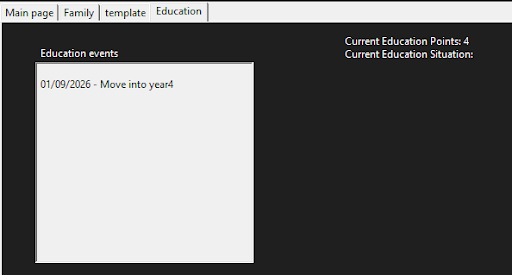
\includegraphics[width=0.8\textwidth]{images/implementation/educationTest3.png}
    \caption{Populated education page on main form}
    \label{fig:implementation-educationTest3}
\end{figure}
\noindent Now, I have the basics working, I need to go through each of the years and add in the events. These will be hard coded for now to save time. If I get more time, I will add in some customisation for this from the players perspective.\\
Shown below is the code for each age of the character. Only shown below is for when the character is 4.
\begin{lstlisting}[language=c, style=csharp, caption=First improvement to the education generation procedure]
case 4:
    //move into reception
    eventArray[controlClass.NextEvent].Category = "Education";
    eventArray[controlClass.NextEvent].DateHappened = dateOfEvent;
    eventArray[controlClass.NextEvent].Description = "Start infant school in Reception.";
    controlClass.NextEvent++;
    mainCharacterScores.EducationScore = mainCharactedScores.EducationScore + randomNumber (1,4);
    break;
\end{lstlisting}

\begin{figure}[H]
    \centering
    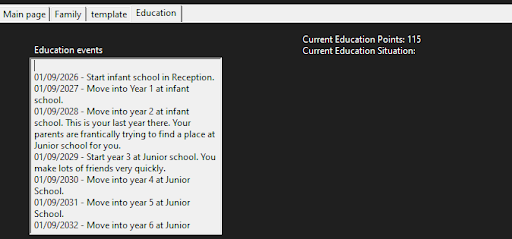
\includegraphics[width=0.8\textwidth]{images/implementation/educationTest4.png}
    \caption{Output of the first improvement of the education system}
    \label{fig:implementation-educationTest4}
\end{figure}
\noindent I got an error during testing where the score value was greater than the max value of the progress bar. This is caused by the progress bar control which displays the education score having a maximum value of 100, and the education score value being set to 101 in the code.\\
To resolve this, I added in an if statement to the update progress bars method.
\begin{lstlisting}[language=c, style=csharp, caption=Improved updateScoresPB procedure]
public void updateScoresPB()
{
    if (mainCharacterScores.EducationScore < prbEducationScore.Maximum && mainCharacterScores.EducationScore > prbEducationScore.Minimum)
    {
        prbEducationScore.Value = mainCharacterScores.EducationScore;
    }
    if(mainCharacterScores.HappinessScore < prbHappinessScore.Maximum && mainCharacterScores.HappinessScore > prbHappinessScore.Minimum)
    {
        prbHappinessScore.Value = mainCharacterScores.HappinessScore;
    }
    if (mainCharacterScores.MedicalScore < prbMedicalScore.Maximum && mainCharacterScores.MedicalScore > prbMedicalScore.Minimum)
    {
        prbMedicalScore.Value = mainCharacterScores.MedicalScore;
    }
    if (mainCharacterScores.LifeScore < prbLifeScore.Maximum && mainCharacterScores.LifeScore > prbLifeScore.Minimum)
    {
        prbLifeScore.Value = mainCharacterScores.LifeScore;
    }
}
\end{lstlisting}
This only updates the progress bar if the education score is less than the maximum value and greater than the minimum value of the progress bar.\\
To progress further with the education generation, I need to now program the choice box form. This will allow the user to select one of three pre-determined options on a new form.

\section{Choice Box Form}
I began by designing the form. All the label controls will be populated programmatically as part of the construction of the form when it is needed; this is why they have been left as the default placeholder text.
\begin{figure}[H]
    \centering
    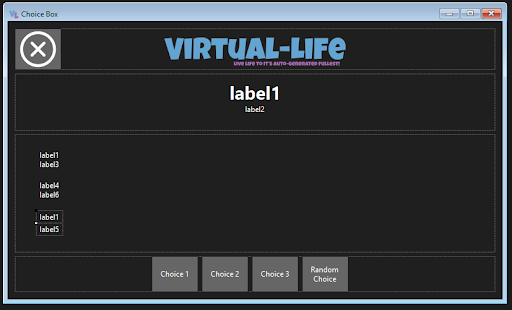
\includegraphics[width=0.8\textwidth]{images/implementation/choiceBox1.png}
    \caption{Choice Box form design}
    \label{fig:implementation-choiceBox1}
\end{figure}
\noindent
Now, I will add the code to pass some test data into the form from my test button on the main game form. Below is the code on \verb|frmMainGameScreen| which calls the choice box.
\begin{lstlisting}[language=c, style=csharp, caption=Code which generates the choice box form and recieves its response]
using (var form = new frmChoiceBox("text here"))
{
    var result = form.ShowDialog();
    if (result == DialogResult.OK)
    {
        string val = form.ReturnValue1; //values preserved after close
        //Do something here with these values
        MessageBox.show(val);
    }
}
\end{lstlisting}
Below is the code on the choice box form which responds to the user pressing \verb|btnChoice1|.
\begin{lstlisting}[language=c, style=csharp, caption=Choice box form code to send the result to where it was called from]
public partial class frmChoiceBox : Form
{
    public string ReturnValue1{get; set; }
    string headerHere;
    public fromChoiceBox(string header)
    {
        InitializeComponent();
        headerHere = header;
    }
    
    private void frmChoiceBox_Load(object sender, EventArgs e)
    {
        MessageBox.show(headerHere);
    }
    
    private void btnChoice1_Click(object sender, EventArgs e)
    {
        this.ReturnValue1 = "Something";
        this.DialogResult = DialogResult.OK;
        this.Close();
    }
}
\end{lstlisting}
When running this, I will expect to see a message box containing "Text here", then the form will appear. When I click the \verb|btnChoice1|, I expect the form to close then a message box to appear containing the word "something".\\
I will now run the program and check what happens.
\noindent First, this message box appears
\begin{figure}[H]
    \centering
    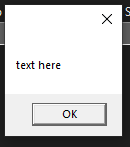
\includegraphics[width=0.3\textwidth]{images/implementation/choiceBox2a.png}
    \caption{Testing choice box 1a}
    \label{fig:implementation-choiceBox2a}
\end{figure}
\noindent Then the form appears
\begin{figure}[H]
    \centering
    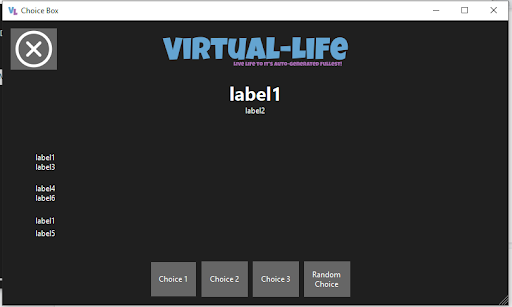
\includegraphics[width=0.8\textwidth]{images/implementation/choiceBox2b.png}
    \caption{Testing choice box 1b}
    \label{fig:implementation-choiceBox2b}
\end{figure}
\noindent Then when I click choice 1, the form closes then this message box appears.
\begin{figure}[H]
    \centering
    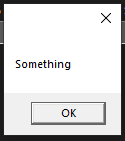
\includegraphics[width=0.3\textwidth]{images/implementation/choiceBox2c.png}
    \caption{Testing choice box 1c}
    \label{fig:implementation-choiceBox2c}
\end{figure}
\noindent This means that this code is working and I can progress onto adding more data passed into the form's constructor.\\
First though, I need to stop the user from selecting anything on the \verb|mainGameScreen| form while the choice box is active. I could either disable all the controls on it or I could just hide the form then re-show it when it\textquotesingle s needed. I'm going to use the latter. To test this, I added in the code to hide the main game form once it had loaded the choice form, then when a response is received from the choice form, re-show the main form.
\begin{lstlisting}[language=c, style=csharp, caption=Code which generates the choice box form and receives its response now with show and hide functions]
using (var form = new frmChoiceBox("text here"))
{
    this.Hide();
    var result = form.ShowDialog();
    this.Show();
    if (result == DialogResult.OK)
    {
        string val = form.ReturnValue1; //values preserved after close
        //Do something here with these values
        MessageBox.show(val);
    }
}
\end{lstlisting}
Now, I need to write the constructor function which will generate the box and process the box. I am writing it this way as I will potentially need to use this form multiple times in one game, meaning I will need to have a reusable piece of code which can be used to generate it.
I added the code needed to send text into and return a value from the choice box. I am expecting a message box to show containing 556 when I close out of the choice box.
\begin{figure}[H]
    \centering
    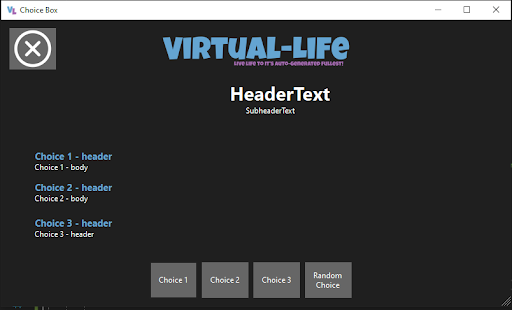
\includegraphics[width=0.8\textwidth]{images/implementation/choiceBox3a.png}
    \caption{Form with data passed into it programmatically}
    \label{fig:implementation-choiceBox3a}
\end{figure}
\begin{figure}[H]
    \centering
    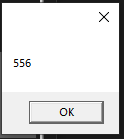
\includegraphics[width=0.3\textwidth]{images/implementation/choiceBox3b.png}
    \caption{Result of pressing button "Choice 1"}
    \label{fig:implementation-choiceBox3b}
\end{figure}
\noindent This means I have a working choice box, for choice 1 at least.
Now I will program the other 4 buttons and test them. I have written the following code to return the value of the button that the user presses.
\begin{lstlisting}[language=c, style=csharp, caption=Code which returns the outcome of the choice box]
private void btnChoice1_Click(object sender, EventArgs e)
{
    this.ReturnValue1 = 1;
    this.DialogResult = DialogResult.OK;
    this.Close();
    
}

private void btnChoice2_Click(object sender, EventArgs e)
{
    this.ReturnValue1 = 2;
    this.DialogResult = DialogResult.OK;
    this.Close();
}

private void btnChoice3_Click(object sender, EventArgs e)
{
    this.ReturnValue1 = 3;
    this.DialogResult = DialogResult.OK;
    this.Close();
}

private void btnRandomChoice_Click(object sender, EventArgs e)
{
    Random rnd = new Random();
    int random = rnd.Next(1, 4);
    this.ReturnValue1 = random;
    this.DialogResult = DialogResult.OK;
    this.Close();
}

private void button1_Click(object sender, EventArgs e)
{
    this.DialogResult = DialogResult.Cancel;
    this.Close();
}
\end{lstlisting}
This is working as expected.\\
Now I have a working choice box which I can feed data into, I need to use it to make some decisions in the game. I am first going to use it when the character turns 4 and has to decide what school to go to. 

\section{Generating names error}
While generating a new game for testing, I came across a bug which is where I have set the upper bound of a random generation too high for the array it is in. This has been a recurring issues with each of the three name generation functions. 
For example, I have given 31 as the upper bound for an array which contains exactly 30 items, when you take into account the zero based nature of arrays in C\#, the error is generated.\\
To fix this error, I have reduced the upper bound to 29. This is working.

\section{Random Generation of Names of Schools}
Now I have the choice box and education system vaguely worked out. I can begin to randomly generate names of schools.
I added the following code to my program

\begin{lstlisting}[language=c, style=csharp, caption=Random generation of schools code]
public int choiceBox(int typeOfChoice, string opt1, string opt2, string opt3)
{
    /*
     * Will need to pass the following into this function and into the choice box form.
     * -type of choice (this will determine the header and subheader text)
     * --> using this rather than passing all information in to simplifiy calls to this function.
     * -opt1
     * -opt2
     * -opt3
     */

    //declare vars used for passing data to choice box
    string headerText = "HeaderText";
    string subheaderText = "SubheaderText";
    string opt1header = "Choice 1";
    string opt1body = opt1;
    string opt2header = "Choice 2";
    string opt2body = opt2;
    string opt3header = "Choice 3";
    string opt3body = opt3;


    //first setup the typeOfChoice
    switch (typeOfChoice)
    {
        case 1:
            //choose infant school
            headerText = "Infant school";
            subheaderText = "Select the infant school you want to spend the next 3 years at";
            break;
        case 2:
            //choose junior school
            headerText = "Junior school";
            subheaderText = "Select the junior school you want to spend the next 4 years at";
            break;
        case 3:
            //choose secondary school
            headerText = "Secondary school";
            subheaderText = "Select the secondary school you want to spend the next 5 years at";
            break;
        case 4:
            //choose college
            headerText = "College";
            subheaderText = "Select the college you want to spend the next 2 years at";
            break;
        default:
            //no option found
            break;
    }

    using (var form = new frmChoiceBox(headerText, subheaderText, opt1header, opt1body, opt2header, opt2body, opt3header, opt3body))
    {

        this.Hide();
        var result = form.ShowDialog();

        this.Show();
        if (result == DialogResult.OK)
        {
            int val = form.ReturnValue1;            //values preserved after close
            //Do something here with these values

            //for example
            
            return (val);
        }
        
    }
    return 0;
}
\end{lstlisting}
When I ran it for the first time, I got the following output. This is erroneous as there is no option for choice 3.
\begin{figure}[H]
    \centering
    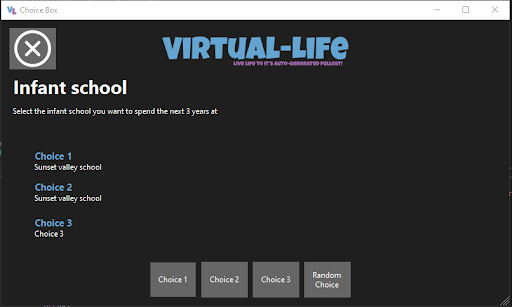
\includegraphics[width=0.8\textwidth]{images/implementation/schoolGen1.png}
    \caption{Output from first run of Random School Generation Code}
    \label{fig:implementation-schoolGen1}
\end{figure}
\noindent I don't mind that choices 1 and 2 are the same as this could add some comedic value to the game.\\
On debugging, I was able to find a typo in the constructor for the choice box form.
\begin{lstlisting}[language=c, style=csharp, caption=Erronious line]
opt3body = opt3h;
\end{lstlisting}
\begin{lstlisting}[language=c, style=csharp, caption=Corrected line]
opt3body = opt3b;
\end{lstlisting}
This correction worked, and I got the result which I was expecting.
\begin{figure}[H]
    \centering
    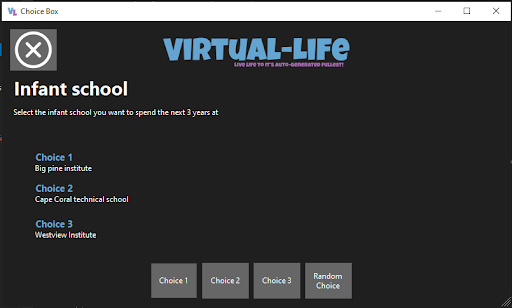
\includegraphics[width=0.8\textwidth]{images/implementation/schoolGen2.png}
    \caption{Correct output from random school name generation code}
    \label{fig:implementation-schoolGen2}
\end{figure}
\noindent Now I have the school name generation worked out for the infant school, I can re-use the functions to generate names of schools for junior and secondary.\\
After adding the code to make this work. I tested this and it works as expected.

\section{Textboxes}
During testing, I was finding it annoying having to scroll down through the events text box and education text box to find the latest event. To solve this, I've changed the code which adds the latest event to the text box from 
\begin{lstlisting}[language=c, style=csharp, caption=Old method of adding text to textbox]
txtEventBox.Text = txtEventBox.Text + Environment.NewLine + eventArray[i].DateHappened.ToShortDateString() + " - " +  eventArray[i].Description;
\end{lstlisting}
to
\begin{lstlisting}[language=c, style=csharp, caption=New method of adding text to a textbox]
txtEventBox.AppendText(Environment.NewLine + eventArray[i].DateHappened.ToShortDateString() + " - " + eventArray[i].Description);
\end{lstlisting}
This has solved my problem and now the textbox scrolls down as the new content is added to it.

\section{Withdraw from Education}
Part of my design is having a way for the character to withdraw from Education.\\
First, I added the button onto the form which will allow this to happen.
\begin{figure}[H]
    \centering
    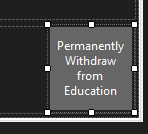
\includegraphics[width=0.2\textwidth]{images/implementation/withdraw1.png}
    \caption{Permanently withdraw from education button}
    \label{fig:implementation-withdraw1}
\end{figure}
\noindent I then added the code to support the button
\begin{lstlisting}[language=c, style=csharp, caption=Withdraw from Education button code]
private void btnEduWithdraw_Click(object sender, EventArgs e)
{
    mainCharacter.InEducation = false;
    eventArray[controlClass.NextEvent].Category = "Education";
    eventArray[controlClass.NextEvent].DateHappened = controlClass.InGameDate;
    eventArray[controlClass.NextEvent].Description = "You permanently withdrew from education. You said it was too boring.";
    controlClass.NextEvent++;
    mainCharacterScores.EducationScore = 0;
}
\end{lstlisting}
I then added an if statement to the checkEducationStatus procedure to check if the character was currently in education or not.\\
This feature works. On the click of age up directly following pressing the withdraw button it gives you the following event:
\begin{figure}[H]
    \centering
    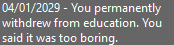
\includegraphics[width=0.2\textwidth]{images/implementation/withdraw2.png}
    \caption{Event generated after pressing Withdraw button}
    \label{fig:implementation-withdraw2}
\end{figure}

\section{Being Born Event}
Currently, when a new game is started, the first event generated states “You were born to parents xxx”. Now I have my parent generation code written, I can add in the parent's names. To do this, I will need to move the code which generates the event from the middle of the new life algorithm to the end, this will make sure that the parents have been generated before their information is inputted to the event array.\\
I also need to change the code which generates the event so it has the names in it.
\begin{lstlisting}[language=c, style=csharp, caption=Improved code for the being born event]
eventArray[controlClass.NextEvent].Category = "Life Event";
eventArray[controlClass.NextEvent].DateHappened = DateTime.Today;
eventArray[controlClass.NextEvent].Description = "You were born to parents " + familyArray[0].FirstName + " and " + familyArray[1].FirstName;
controlClass.NextEvent++;
\end{lstlisting}
This worked the first time I ran the code and gave me the result I was expecting.
\begin{figure}[H]
    \centering
    
\includegraphics[width=0.2\textwidth]{images/implementation/birthEvent1.png}
    \caption{Event generated after being born}
    \label{fig:implementation-birthEvent1}
\end{figure}

\section{Generate Event Procedure}
It is quite laborious having to write 4 lines of code to generate a single event. As I am using this more and more, I am going to write a procedure which will do it for me.\\
I used my standard 4 lines of code and copied them into a procedure then wrote the test code to test it with.
\begin{lstlisting}[language=c, style=csharp, caption=Code for generateEvent procedure]
public void generateEvent(string category, string content, DateTime date)
{
    eventArray[controlClass.NextEvent].Category = category;
    eventArray[controlClass.NextEvent].DateHappened = date;
    eventArray[controlClass.NextEvent].Description = content;
    controlClass.NextEvent++;
}
\end{lstlisting}
This worked the first time I ran it and produced the result I was expecting.

\section{Scores}
Now I have some of the bigger elements of the game programmed, I can start thinking more about the scores. To do this, I need to generate modifiers; this is where the \verb|ControlClass| will be used to store these modifiers. Then I will be able to write my \verb|lifeScore| algorithm.\\
First, I am going to change how the scores are initially assigned to the character. The character\textquotesingle s job score and education score will start off at zero, as in real life this is how it works. For now, I am also setting the medical score to 0 as I still need to write the algorithm which will calculate this and generate conditions for the characters. Happiness score will still be randomly generated as this is relatively random in life. After making these changes, this is what the declaration of the main character scores looks like:
\begin{lstlisting}[language=c, style=csharp, caption=Initial score assignment to character]
mainCharacterScores.EducationScore = 0;
mainCharacterScores.JobScore = 0;
mainCharacterScores.HappinessScore = rnd.Next(0, 101);
mainCharacterScores.MedicalScore = 0;
mainCharacterScores.LifeScore = 0;
\end{lstlisting}
Now I am going to change the maximum value of each of the progress bar controls using the control property panel in Visual Studio to 1000, this will give me more room to manipulate the value.
\begin{lstlisting}[language=c, style=csharp, caption=Original education score calculator]
public void calculateEducationScore()
{
    //Calculate the education score based off of the current score and the modifier
    //1 in 8 chance of the score being decreased rather than being increased. When decreased, needs to go down a fair chunk.

    int randomReturn = randomNumber(1, 8);
    if (randomReturn == 6)
    {
        //Decrease
        mainCharacterScores.EducationScore = mainCharacterScores.EducationScore - controlClass.EduScorePlus;
    }
    else
    {
        //increase 
        //1 in 2 chance of modifier being upped by 0.3 of the current modifier.
        int randomReturn1 = randomNumber(1, 3);
        if(randomReturn1 == 1)
        {
            //normal modifier
            mainCharacterScores.EducationScore = mainCharacterScores.EducationScore + controlClass.EduScorePlus;
        }
        else if (randomReturn1 == 2)
        {
            //increased modifier
            int plus = (int)Math.Round(controlClass.EduScorePlus * 0.3);
            mainCharacterScores.EducationScore = mainCharacterScores.EducationScore + plus;
        }
    }

}
\end{lstlisting}
The first time I ran this code, the education score stayed extremely low the entire time. To combat this, I am going to change the decrease check to a chance of 1 in 30 and increase the original eduscoreplus to 10.
This has improved the situation somewhat. I got a score of 92 at the point at which the character left school. I am still not happy though, as I was hoping it would be possible to max out the progress bar and keep scoring more. I am going to increase the beginning eduscoreplus value again, this time to 50.
Again, this didn't produce the answer I wanted. So I doubled that value, giving me an eduscoreplus value of 100. This worked much better and produced me a score of 840 when the character turned 18.
I am satisfied with this algorithm and can now begin to look at the happiness score algorithm.\\
The happiness score is going to be a mixture of various factors which will be combined together to create one score. Initially, the factors I am going to start with is an age based calculation, with the thinking that when a person is younger they will be happier (however, there will be a chance that this is a low score)\\
I will first write the function to update the score.
\begin{lstlisting}[language=c, style=csharp, caption=Happiness score calculation algorithm]
public void updateHappinessScore(int externalModifier)
{
    //add to the current happiness score the generic value to increse by plus a modifier
    mainCharacterScores.HappinessScore = mainCharacterScores.HappinessScore + controlClass.HappinessScorePlus + externalModifier;
    
}
\end{lstlisting}
On running this code, it isn't increasing the value. On investigation, I have found that I didn't change a line of code in the generate initial value section.
\begin{lstlisting}[language=c, style=csharp, caption=Generation of happiness score modifier algorithm]
public int generateHappinessScorePlusVal()
{
    //generate the happinessScorePlus value.
    //random chance that this is a low plus score initially, 
    Random rnd = new Random();
    int randomChance = rnd.Next(1, 30);
    int val = 10;
    if (randomChance == 4)
    {
        //goes up slowly
        val = rnd.Next(1, 10);
    }
    else
    {
        //goes up quickly
        val = rnd.Next(11, 30);
    }
    return 0;
}
\end{lstlisting}
The return value shouldn't be set to 0, it should be set to the integer val.\\
This is now working and on running the code, I realised that the value is increasing far too quickly. To solve this, I changed the goes up quickly value to 11-30. This is working much better, with a considerably slower increase allowing me to change factors more throughout the rest of the implementation stage.\\
Now, I need to add the code which will decrease the happiness score a random amount when a family member dies.
\begin{lstlisting}[language=c, style=csharp, caption=Code to reduce the main character happiness score once a family member has died]
//now reduce mc happiness score
mainCharacterScores.HappinessScore = mainCharacterScores.HappinessScore - randomNumber(1, 100);
\end{lstlisting}
For now, this is all the implementation of scores that I can do. To be able to implement the medical and job scores, I will need to to write the medical condition algorithms and job algorithms.

\section{More displaying of scores}
The progress bars which I am using to display the scores are good at a visual representation of the max and min values and where the player is; but they don't give accurate representations. To solve this, I am going to use a tooltip which will display the score.\\
This is the result of the code shown below.
\begin{figure}[H]
    \centering
    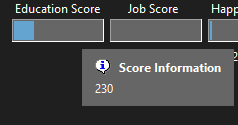
\includegraphics[width=0.4\textwidth]{images/implementation/scoresDisplay1.png}
    \caption{Scores progress bar with ToolTip visible}
    \label{fig:implementation-scoresDisplay1}
\end{figure}
This is the code which is run when the progress bars are updated.
\begin{lstlisting}[language=c, style=csharp, caption=Code to populate ToolTips showing score information]
ttMainToolTip.SetToolTip(prbEducationScore, prbEducationScore.Value.ToString());
ttMainToolTip.SetToolTip(prbHappinessScore, prbHappinessScore.Value.ToString());
ttMainToolTip.SetToolTip(prbJobScore, prbJobScore.Value.ToString());
ttMainToolTip.SetToolTip(prbLifeScore, prbLifeScore.Value.ToString());
ttMainToolTip.SetToolTip(prbMedicalScore, prbMedicalScore.Value.ToString());
\end{lstlisting}

\section{Disable clickables}
During testing, I realised that I have some clickable items (buttons etc) which are still enabled when the main character dies. To solve this, I am going to write a procedure which will disable all the clickable controls when it is run.\\
To do this, I will need a new procedure, shown below.
\begin{lstlisting}[language=c, style=csharp, caption=Disable clickables subroutine]
public void disableClickables()
{
    //procedure to disable all clickable elements on this form, for use when the main char dies.
    //There is no way to reverse this.

    btnAgeUp.Enabled = false;
    btnEduWithdraw.Enabled = false;
}
\end{lstlisting}
As the comments say, there is no way to overturn this procedure as this is only to be used at the very end of the game when the character is dead.\\
This worked the first time I tried this, shown below
\begin{figure}[H]
    \centering
    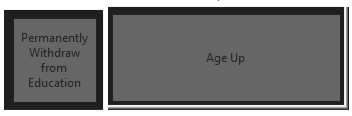
\includegraphics[width=0.4\textwidth]{images/implementation/disableClick1.jpg}
    \caption{Buttons disabled after the procedure above has been run}
    \label{fig:implementation-disableClick1}
\end{figure}
\noindent I am satisfied with this procedure as it works as expected.

\section{About Form}
This form is used to credit the assets I have downloaded from the internet. There are no programmatically elements to it apart from opening it. All design will be done in Visual Studio's designer.\\
Below is the form.
\begin{figure}[H]
    \centering
    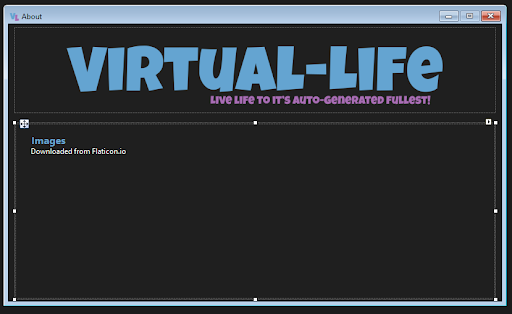
\includegraphics[width=0.8\textwidth]{images/implementation/aboutForm.png}
    \caption{About form design}
    \label{fig:implementation-aboutForm}
\end{figure}

\section{Crimes}
Now I need to add the code in which will let the player generate a random crime for their player to commit. It will be a very basic system, which gives the player no choice on what crime they commit and all the sentences will be between 1 and 12 years community service. For added humour, I won't be disabling this button until the character reaches a certain age as I feel it would be more amusing to have a 2 year old stealing a car.\\
See below for the code which runs the page on the tab control.
\begin{lstlisting}[language=c, style=csharp, caption=Procuedres which are run when the "Comit Random Crime" button is pressed]
private void btnCriCommitCrime_Click(object sender, EventArgs e)
{
    //first generate new crime then time of community service for it. 

    string[] crimes = { "Burgle a shop", "Steal a car", "Pirate a DVD" };
    int crimesLength = crimes.Length;
    int rand = randomNumber(0, crimesLength);
    int years = randomNumber(1, 12);
    string crimeText = "You committed a crime " + crimes[rand] + " and you recieved " + years.ToString() + " years community service.";
    generateEvent("Crime", crimes[rand], controlClass.InGameDate);
    updateCrimes();
}

public void updateCrimes()
{
    txtCriCrimeEvents.ResetText();
    for (int i = 0; i < controlClass.NextEvent; i++)
    {
        if (eventArray[i].Category == "Crimes")
        {
            txtCriCrimeEvents.Text = txtCriCrimeEvents.Text + Environment.NewLine + eventArray[i].DateHappened.ToShortDateString() + " - " + eventArray[i].Description;
        }

    }
}
\end{lstlisting}
This initially didn't work as expected as the crime only textbox doesn't show crimes however the main event box does. To rectify the issue with the crime only box, I corrected the line of code in \verb|updateCrimes()| in the if statement from “Crimes” to “Crime”. This works and produces the results I want.
\begin{figure}[H]
    \centering
    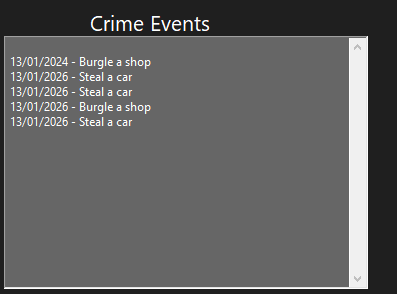
\includegraphics[width=0.4\textwidth]{images/implementation/crime1.png}
    \caption{Crime event box}
    \label{fig:implementation-crime1}
\end{figure}

\section{Customising Character}
To start working on this section, I need to design the form.
\begin{figure}[H]
    \centering
    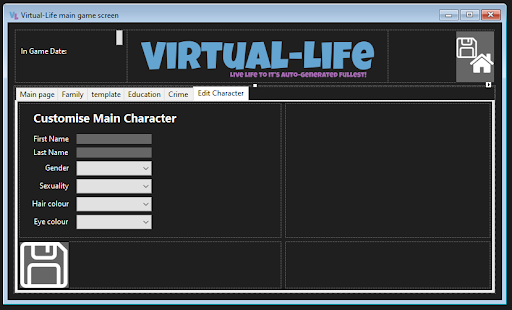
\includegraphics[width=0.8\textwidth]{images/implementation/customise1.png}
    \caption{Customise character options}
    \label{fig:implementation-customise1}
\end{figure}
\noindent This just has the customisation options at the moment and the save button. I still need to add the end life section to the right hand side of the screen. 
Now I need to add the code which will unlock these options once the main character has turned 13.
\begin{lstlisting}[language=c, style=csharp, caption=Yearly Check subroutine]
public void yearlyCheck()
{
    //this is a place which will run every time the mc ages up. If they are older than the specified age then will run code in relevant section.

    if(mainCharacter.Age >= 13)
    {
        //'unlock' character customisation screen.
        txtEditFirstName.Enabled = true;
        txtEditLastName.Enabled = true;
        cboEditGender.Enabled = true;
        cboEditSexuality.Enabled = true;
        cboEditEyeColour.Enabled = true;
        cboEditHairColour.Enabled = true;
    }
}
\end{lstlisting}
I have done this by writing a new procedure yearlyCheck() which gets run every time the player clicks age up. It will force the character customisation options to be enabled once the character turns 13. 
Next, I need to write the code which will populate these controls with the current information which the main character has.
\begin{lstlisting}[language=c, style=csharp, caption=Subroutine to update character customisaiton options]
public void updateCharCustomisationOptions()
{
    //fill all the Character Customisation option controls with current information from main char object
    txtEditFirstName.Text = mainCharacter.FirstName;
    txtEditLastName.Text = mainCharacter.LastName;
    cboEditGender.Text = mainCharacter.Gender;
    cboEditSexuality.Text = mainCharacter.Sexuality;
    cboEditHairColour.Text = mainCharacter.HairColour;
    cboEditEyeColour.Text = mainCharacter.EyeColour;
}
\end{lstlisting}
This procedure is called as part of the \verb|updateForms| procedure so it will be called every time age up is clicked.\\
Now I need to write the save button algorithm.
\begin{lstlisting}[language=c, style=csharp, caption=Save character customisation procedure]
public void saveCharCustomisationOptions()
{
    //if the contents of the text boxes etc is NOT null and is different to the current contents of the main character object, then it needs to be written into the object

    //start with the first name
    if(txtEditFirstName.Text != null && txtEditFirstName.Text != mainCharacter.FirstName)
    {
        mainCharacter.FirstName = txtEditFirstName.Text;
    }
    //next - do the last name
    if(txtEditLastName.Text != null && txtEditLastName.Text != mainCharacter.LastName)
    {
        mainCharacter.LastName = txtEditLastName.Text;
    }
    if(cboEditGender.Text != null && cboEditGender.Text != mainCharacter.Gender)
    {
        mainCharacter.Gender = cboEditGender.Text;
    }
    if(cboEditSexuality.Text != null && cboEditSexuality.Text != mainCharacter.Sexuality)
    {
        mainCharacter.Sexuality = cboEditSexuality.Text;
    }
    if(cboEditHairColour.Text != null && cboEditHairColour.Text != mainCharacter.HairColour)
    {
        mainCharacter.HairColour = cboEditHairColour.Text;
    }
    if(cboEditEyeColour.Text != null && cboEditEyeColour.Text != mainCharacter.EyeColour)
    {
        mainCharacter.EyeColour = cboEditEyeColour.Text;
    }
}
\end{lstlisting}
This half worked the first time I tried it. The edit aspect worked and the main display tab updated as I expected it to, however when I tried a null entry, the program allowed this to happen.
\begin{figure}[H]
    \centering
    
\includegraphics[width=0.4\textwidth]{images/implementation/customise2.png}
    \caption{Textbox on Customisation form}
    \label{fig:implementation-customise2}
\end{figure}

\begin{figure}[H]
    \centering
    
\includegraphics[width=0.4\textwidth]{images/implementation/customise3.png}
    \caption{Main info point on main game screen}
    \label{fig:implementation-customise3}
\end{figure}
\noindent To resolve this, I changed \verb|null| to \verb|""|. This worked and I now have a working character customisation page.\\
Next, I need to add the end life button. This will still generate a random reason for death.
First, I added the controls to the form then I added the code which will power it.\\
\begin{figure}[H]
    \centering
    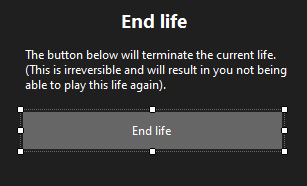
\includegraphics[width=0.4\textwidth]{images/implementation/endlife1.png}
    \caption{Button which ends the main characters life}
    \label{fig:implementation-endlife1}
\end{figure}
\begin{lstlisting}[language=c, style=csharp, caption=End life algorithm]
private void btnEndLife_Click(object sender, EventArgs e)
{
    DialogResult dialogResult = MessageBox.Show("Are you sure you want to end this life?", "End life", MessageBoxButtons.YesNo);
    if (dialogResult == DialogResult.Yes)
    {
        killMainCharacter();
    }
    else if (dialogResult == DialogResult.No)
    {
        //do something else
    }
}
\end{lstlisting}
As you can see from the code, it calls the same procedure that would be called if the main character was to die randomly.
\begin{figure}[H]
    \centering
    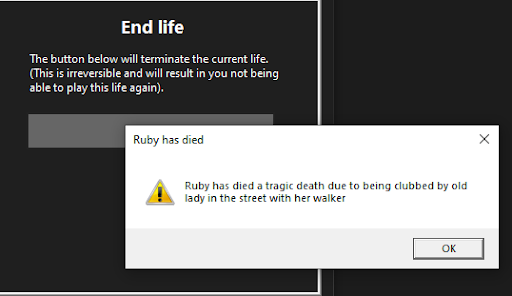
\includegraphics[width=0.6\textwidth]{images/implementation/endlife2.png}
    \caption{Output from pressing the end life button}
    \label{fig:implementation-endlife2}
\end{figure}
\noindent This worked as expected.

\section{Jobs}
The next part of the game which I am going to program is the jobs and employment feature.
To start off, I am going to follow my design and create a new tab page on the main tab control with the controls outlined in my design.
\begin{figure}[H]
    \centering
    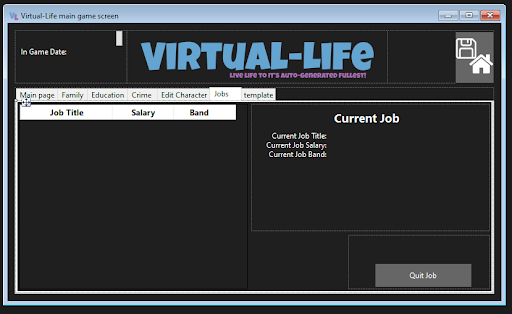
\includegraphics[width=0.8\textwidth]{images/implementation/jobs1.png}
    \caption{Design of the jobs form}
    \label{fig:implementation-jobs1}
\end{figure}
\noindent I then began to write the algorithm to generate jobs.
\begin{lstlisting}[language=c, style=csharp, caption=Algorithm to generate jobs]
 public Job generateJob (int band)
{
    string[] band1Job = { "Cleaner", "Wearhouse opperative", "Grocery picker", "Sahara delivery driver", "Burger flipper", "Hospital porter", "Community care worker", "Care assistant", "Handyperson", "Nursery assistant" };
    string[] band2Job = { "College security guard", "Pet groomer", "Engineer", "Secretary", "Line cook", "Plumber", "Cleaning company owner", "HR advisor", "Vehicle Technician", "Tanker driver" };
    string[] band3Jobs = { "Supervisor", "Senior Vehicle Technician", "Head of Resources", "Product manager", "Web developer", "Comms manager", "Software engineer", "Project manager", "Site manager", "Sales Director" };
    string[] band4Jobs = { "Store manager", "Finance Manager", "Site supervisor", "Nursing home manager", "IT Solutions Architect", "Senior API Developer", "Electrical Installation Lecturer", "Matron", "Defects manager", "Family Lawyer" };
    string[] band5Jobs = { "CEO", "Retail park manager", "Hotel manager", "Specialty doctor", "User interface designer", "SQL Developer", "DevOps engineer", "Senior Software consultant", "Executive head teacher", "Hospital director" };
    Job newJob = new Job();
    Random rnd = new Random();
    switch (band)
    {
        case 1:
            Salary = 17000;
            Band = 1;
            JobTitle = band1Job[rnd.Next(1, 9)];
            break;
        case 2:
            Salary = 34000;
            Band = 2;
            JobTitle = band2Job[rnd.Next(1, 9)];
            break;
        case 3:
            Salary = 51000;
            Band = 3;
            jobTitle = band3Jobs[rnd.Next(1, 9)];
            break;

        case 4:
            Salary = 68000;
            Band = 4;
            jobTitle = band4Jobs[rnd.Next(1, 9)];
            break;
        case 5:
            Salary = 150000;
            Band = 5;
            jobTitle = band5Jobs[rnd.Next(1, 9)];
            break;
    }
    return newJob;
}
\end{lstlisting}
I wrote some test code which would use a test button to generate a job and output the job title in a message box.
\begin{lstlisting}[language=c, style=csharp, caption=Procedure to call the generateJob function]
private void btnTestButton_Click(object sender, EventArgs e)
{
    Job newJob = new Job();
    newJob.generateJob(1);
    MessageBox.show(newJob.JobTitle);
}
\end{lstlisting}
When I ran the code, it gave me the following result; this means that my job generation code is working.
\begin{figure}[H]
    \centering
    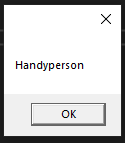
\includegraphics[width=0.2\textwidth]{images/implementation/jobs2.png}
    \caption{Result from pressing test button}
    \label{fig:implementation-jobs2}
\end{figure}
\noindent Next, I need to write the algorithm which once the main character turns 18 generates band 1 jobs and populates the data grid view which they will be stored in. This is going to be done using a procedure - reshuffle Jobs. This is going to also be able to be called from the button which will reshuffle jobs. This button will initially be disabled, however once the main character turns 18, it will be enabled (in the same way as the edit character controls).
To start writing \verb|reshuffleJobs|, I will first generate the array of Job objects each containing different band jobs.It will then output these jobs to a \verb|DataGridView| control.
\begin{lstlisting}[language=c, style=csharp, caption=Reshuffle available jobs algorithm]
public void reshuffleJobs(int band)
{
    //first generate the jobs
    int maxNumb = 10;
    for (int i = 0; i < maxNumb; i++)
    {
        Job tempJob = new Job(); //make new instance of the object
        tempJob.generateJob(band); 
        availableJobs[i] = tempJob; //transfer the temp object into the array.
    }

    //now populate data grid view
    //first have to clear it
    dgvEmpAvailableJobs.Rows.Clear();
    dgvEmpAvailableJobs.Refresh();

    //use code from openldbws app to populate dgvEmpAvailableJobs

    //first, set var for which column contains which data
    int jtCol = 0;
    int salCol = 1;
    int bandCol = 2;

    //now loop through familyArray and populate dgvEmpAvailableJobs
    //as jobs are only ever generated and populated here - can use max number from job generation loop for loop here

    for (int x = 0; x < maxNumb; x++)
    {
        if (availableJobs[x].JobTitle != null)
        {
            int i = dgvEmpAvailableJobs.Rows.Add();
            dgvEmpAvailableJobs.Rows[i].Cells[jtCol].Value = availableJobs[x].JobTitle;
            dgvEmpAvailableJobs.Rows[i].Cells[salCol].Value = availableJobs[x].Salary;
            dgvEmpAvailableJobs.Rows[i].Cells[bandCol].Value = availableJobs[x].Band;
        }
    }
}
\end{lstlisting}
Which look like this
\begin{figure}[H]
    \centering
    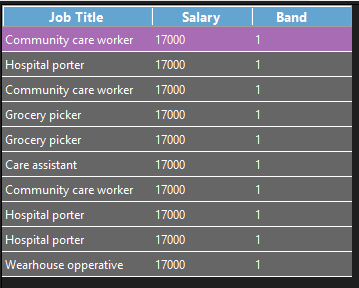
\includegraphics[width=0.5\textwidth]{images/implementation/jobs3.png}
    \caption{Output of DataGridView control}
    \label{fig:implementation-jobs3}
\end{figure}
\noindent This worked first time as I copied and altered the code from the generation and population of the \verb|genericFamilyMember| object array and display for that.\\
Now I need to be able to “apply” for the job and display information about the job. First I added the apply button to the main form, then I wrote the code which will populate the label controls (displaying the current job information) and save the job which the main character has selected to the main character object.
\begin{lstlisting}[language=c, style=csharp, caption=Applying for job and updating job information procedures]
public void updateCurrentJobInformation()
{
    lblJobCurrentJobBand.Text = "Current Job Band: " + mainCharacter.JobBand.ToString();
    lblJobCurrentJobTitle.Text = "Current Job Title: " + mainCharacter.JobTitle.ToString();
    lblJobCurrentJobSalary.Text = "Current Job Salary: " + mainCharacter.JobSalary.ToString();

}

private void btnJobApplyForJob_Click(object sender, EventArgs e)
{
    mainCharacter.JobTitle = dgvEmpAvailableJobs.SelectedCells[0].Value.ToString();
    mainCharacter.JobSalary = Int32.Parse(dgvEmpAvailableJobs.SelectedCells[1].Value.ToString());
    mainCharacter.JobBand = Int32.Parse(dgvEmpAvailableJobs.SelectedCells[2].Value.ToString());
    updateCurrentJobInformation();
}
\end{lstlisting}
When I ran this for the first time, I got the following error: Object reference not set to an instance of an object with the displaying \verb|JobTitle| line highlighted.\\
To resolve this, I removed the \verb|.ToString()| method from the attributes which were already strings.
This worked, however I hadn't added the attribute titles to the code, which means it gets removed when the button is pressed. This gives me the result of
\begin{figure}[H]
    \centering
    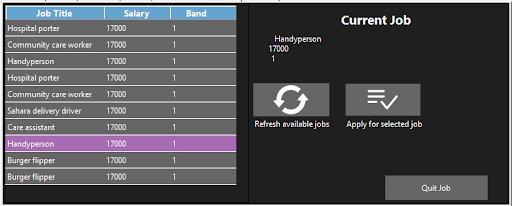
\includegraphics[width=0.8\textwidth]{images/implementation/jobs4.png}
    \caption{Job page of main form (without label titles)}
    \label{fig:implementation-jobs4}
\end{figure}
\noindent Now I\textquotesingle ve added in the label titles, I get
\begin{figure}[H]
    \centering
    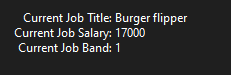
\includegraphics[width=0.4\textwidth]{images/implementation/jobs5.png}
    \caption{Correct display of job information}
    \label{fig:implementation-jobs5}
\end{figure}
\noindent I then tried to click on the apply for select job before I had loaded the available jobs, this resulted in the following error.
\begin{figure}[H]
    \centering
    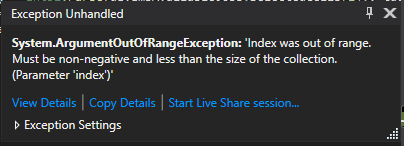
\includegraphics[width=0.5\textwidth]{images/implementation/jobs6.png}
    \caption{Error from not selecting a job before applying for it}
    \label{fig:implementation-jobs6}
\end{figure}
\noindent To solve this, I added a \verb|Try-Catch| block with the exception handled by displaying a message to the user.
\begin{lstlisting}[language=c, style=csharp, caption=Apply for job procedure now with try-catch block]
 private void btnJobApplyForJob_Click(object sender, EventArgs e)
{
    try
    {
        mainCharacter.JobTitle = dgvEmpAvailableJobs.SelectedCells[0].Value.ToString();
        mainCharacter.JobSalary = Int32.Parse(dgvEmpAvailableJobs.SelectedCells[1].Value.ToString());
        mainCharacter.JobBand = Int32.Parse(dgvEmpAvailableJobs.SelectedCells[2].Value.ToString());
        mainCharacter.InJob = true;
        generateEvent("Job", "You applied for and got the job: " + mainCharacter.JobTitle, controlClass.InGameDate);
        updateCurrentJobInformation();
    } catch(Exception)
    {
        MessageBox.Show("Please select a job before applying for it.");
    }
}
\end{lstlisting}
This results in
\begin{figure}[H]
    \centering
    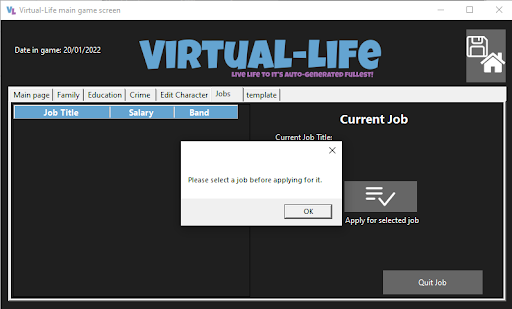
\includegraphics[width=0.8\textwidth]{images/implementation/jobs7.png}
    \caption{Result of applying for job without selecting a job after adding try-catch block}
    \label{fig:implementation-jobs7}
\end{figure}
\noindent Now I need to add the quit job code. As this button will be enabled even if the main character isn't currently in a job, I will use a try catch block again; to catch any exceptions.
\begin{lstlisting}[language=c, style=csharp, caption=Quit job algorithm]
private void button1_Click(object sender, EventArgs e) //quit job
{
    try
    {
        mainCharacter.JobTitle = "";
        mainCharacter.JobSalary = 0;
        mainCharacter.JobBand = 0;
        mainCharacter.InJob = false;
        mainCharacter.JobCurrentDuration = 0;
        generateEvent("Job", "You quit your job", controlClass.InGameDate);
    }
    catch (Exception)
    {
        MessageBox.Show("Please make sure you have a job before you try to quit it.");
    }
    updateCurrentJobInformation();
}
\end{lstlisting}
This worked as expected and gave me the results I wanted.
\begin{figure}[H]
    \centering
    \includegraphics[width=0.2\textwidth]{images/implementation/jobs8.png}
    \caption{Result of quitting a job in the events box}
    \label{fig:implementation-jobs8}
\end{figure}
\noindent Now that I have obtain and quit job code working, I need to write the job progression algorithms. This algorithm is going to work by looking at the \verb|JobCurrentTime| attribute of the main character and if the character has been in their current job for over a certain time then they will be offered the next band of job up. To start this algorithm, I will change the generate job procedure so if the main character has been in a job for less than 5 years the game will generate band 1 jobs.
This is the event handler code for when the button is pressed:
\begin{lstlisting}[language=c, style=csharp, caption=Start of the Reshuffle Job Board algorithm]
private void btnJobReshuffleJobBoard_Click(object sender, EventArgs e)
{
    if(mainCharacter.JobCurrentDuration < 5)
    {
        //can only get band 1 job
        reshuffleJobs(1);
    }
}
\end{lstlisting}
This worked so I can now add the second band code
\begin{lstlisting}[language=c, style=csharp, caption=Second iteration of the reshuffle job board algorithm]
private void btnJobReshuffleJobBoard_Click(object sender, EventArgs e)
{
    if(mainCharacter.JobCurrentDuration <= 5)
    {
        //can only get band 1 job
        reshuffleJobs(1);
    }
    else if (mainCharacter.JobCurrentDuration >=6 && mainCharacter.JobCurrentDuration <= 14)
    {
        //get band 2 job
        reshuffleJobs(2);
    }
}
\end{lstlisting}
This is also working and generating band 1 jobs while the main character has had a job for under 6 years then generating a band 2 job after that. As this is working, I can write the code to generate the rest of the bands of jobs.\\
This is working and producing the results I expect it to.\\
The next part of the jobs algorithm I need to program is the salary calculation This algorithm will be run every time the main character ages up, so the first thing which I need to do is check if the main character currently has a job. I am then able to write the code which will take the current salary, band and duration of which the main character has been in a job. \\
Below is the algorithm which will calculate the salary
\begin{lstlisting}[language=c, style=csharp, caption=Calculate job salary algorithm]
public void calculateSalary()
{
    Random rnd = new Random();
    //algorithm to generate the salary of the main character
    //needs to take into consideration the current band of job, base band of that salary and how long the mc has been in that job
    int salary = mainCharacter.JobSalary;
    int band = mainCharacter.JobBand;
    int duration = mainCharacter.JobCurrentDuration;

    if(mainCharacter.InJob == true)
    {
        //mc is in job so can now calc salary.
        int increaseAmount = rnd.Next(0, (band*duration));
        mainCharacter.JobSalary = salary + increaseAmount;
    }
}
\end{lstlisting}
To test this, I ran the program and found that the increases are too marginal for the game to be fun. I will need to increase the max increase amount by a factor of 10.
\begin{lstlisting}[language=c, style=csharp, caption=Salary increase amount calculation]
int increaseAmount = rnd.Next(0, (band*duration)*10);
\end{lstlisting}
This still isn't increasing the salary as much as I would like it to, so I am going to change the increase factor to 50. This is working much better and I am now happy with the salary calculation and salary increase algorithms.
Now I have built the jobs segment of the game, I need to remove the test settings, so players can only get jobs when they turn 18. I am going to do this in the same way that I did for the character customisation options, making the controls on the form default to be disabled, then every time age up is clicked they are enabled.
\begin{lstlisting}[language=c, style=csharp, caption=Age restriction for the jobs algorithms]
if (mainCharacter.Age >= 18)
{
    //'unlock' character job options
    btnJobApplyForJob.Enabled = true;
    btnJobQuitJob.Enabled = true;
    btnJobReshuffleJobBoard.Enabled = true;
}
\end{lstlisting}
This is working as I want it to.
Finally, the job score will simply be the duration which you have had the job for.
I have put the code for this in the \verb|updateCurrentJobInformation| procedure as this is both run every time a change is made to the employment situation and whenever the main character is aged up.
\begin{lstlisting}[language=c, style=csharp, caption=JobScore algorithm]
mainCharacterScores.JobScore = mainCharacter.JobCurrentDuration*4;
prbJobScore.Value = mainCharacterScores.JobScore;
\end{lstlisting}

\section{Medical}
This is going to be a very much behind the scenes algorithm which is going to randomly assign the medical score as well as enter some messages into the events box denoting what has happened medically. There will be no player interaction with this algorithm.
It will first get the main character\textquotesingle s current medical score, depending on what this is, the algorithm will generate a medical condition which will have a 5\% chance of affecting the main character. All the medical conditions generated will either be life-long or will never need to be referenced again, therefore I can save some processing by not needing to keep detailed information about each medical condition, meaning the game will be more lightweight to run.
Before I can write the algorithm, I'm going to have to change how the medical score is assigned when a new game is generated, it will have to be set to 100 not 0.
\begin{lstlisting}[language=c, style=csharp, caption=Medical score algorithms]
public void generateMedicalScore()
{
    Random rnd = new Random();
    int currentMedScore = mainCharacterScores.MedicalScore;
    if(currentMedScore == 100)
    {
        //has perfect health, 1/10 chance of it being lowered so can then be diseased.
        int chance = rnd.Next(0, 11);
        if(chance == 5)
        {
            currentMedScore = 99;
        }

    }
    if(currentMedScore < 100)
    {
        //can be diseased. 1 in 20 chance of getting disease
        int chance1 = rnd.Next(0, 21);
        if(chance1 == 12)
        {
            //is gonna be diseased
            string condition = getMedicalCondition();

            generateEvent("Medical","You " + condition, controlClass.InGameDate);

            mainCharacterScores.MedicalScore = mainCharacterScores.MedicalScore - rnd.Next(0, 50);

        }
    }
}

public string getMedicalCondition()
{
    string[] medicalConditions = {"broke your arm", "broke your leg", "stubbed your toe" };
    Random rnd = new Random();

    string returnString = medicalConditions[rnd.Next(0, medicalConditions.Length)];
    return returnString;
}
\end{lstlisting}
I tested this algorithm and it worked.
\begin{figure}[H]
    \centering
    \includegraphics[width=0.3\textwidth]{images/implementation/medical1.png}
    \caption{Result of medical condition generation}
    \label{fig:implementation-medical1}
\end{figure}
\noindent Now I just need to change the medical score value to 1000 and increase the decrease med score value.

\section{Partners}
The final main element of the game I need to program is the partner and courtship element. The courtship element will be an extremely simplified version of real life as every couple has a different path.
To start off with, I need to program the generation of a potential partner. There will be no lower age limit on this and the partner will have to be within 2 years of the main character. This will be generated in much the same way as the generic family members when a new game is created.
This is the code I have written in the main game screen form which is run whenever the button to generate potential partners is pressed.
\begin{lstlisting}[language=c, style=csharp, caption=Code to generate more potential partners]
private void btnParGenMore_Click(object sender, EventArgs e)
{
    generateAndPopulateMorePartners();
}

public void generateAndPopulateMorePartners()
{
    //Now create family members
    for (int i = 0; i < 10; i++)
    {
        DetailedCharacter tempFamily = new DetailedCharacter(); 
        tempFamily.generateDetailedChar(); 
        MessageBox.Show(tempFamily.FirstName);
    }
\end{lstlisting}
This calls the function in the detailed person class which looks like this.
\begin{lstlisting}[language=c, style=csharp, caption=Detailed char class code to generate a partner]
public DetailedCharacter generateDetailedChar()
{
    DetailedCharacter potential = new DetailedCharacter();
    FirstName = "Dave";
    return potential;
}
\end{lstlisting}
For testing, I have just programmed the first name to be “Dave”. This will allow me to make sure that everything is being called properly before I move onto the next part.\\
To test this so far, I can click the generate button and run the code.
\begin{figure}[H]
    \centering
    \includegraphics[width=0.2\textwidth]{images/implementation/partners1.png}
    \caption{Outcome from pressing generate button}
    \label{fig:implementation-partners1}
\end{figure}
\noindent This gave me the outcome which I expected. I will now move onto the display feature of the potential partners.
To do this, I will need to write the code which will add the generated temporary object to the array and write the code which will output the information to the user. The later I already have as I have been using \verb|DataGridViews| lots throughout the project, and the former I have in a different state which I can use here.\\
After running the code and once again confirming that the correct number of \verb|Dave|s appeared, the \verb|DataGridView| was populated as follows, confirming that the code is working this far.
\begin{figure}[H]
    \centering
    \includegraphics[width=0.4\textwidth]{images/implementation/partners2.png}
    \caption{Initial test of the data grid view used to show potential partners}
    \label{fig:implementation-partners2}
\end{figure}
Now I have the display working, I have a way to test the development of the different potential partners. The different combinations of sexuality and gender will be generated within the detailed character class.\\
Initially, I will be using a straight woman to start development.
\begin{lstlisting}[language=c, style=csharp, caption=Code to generate potential partners for a straight woman]
public DetailedCharacter generateDetailedChar(string gender, string sexuality, DateTime today)
{
    DetailedCharacter potential = new DetailedCharacter();

    if (gender == "Female")
    {
        if (sexuality == "Straight")
        {
            //generate a man
            FirstName = genMFN();
            LastName = genLN();
            Sexuality = "Straight";
            Gender = "Male";
            LivingStatus = true;
            DateOfBirth = today.AddDays(-rnd.Next(5840, 14600));
            Age = calcAge(DateOfBirth);
        }
    }
    FirstName = "Dave";
    return potential;
\end{lstlisting}
This worked as expected except for the fact I had left a line of debug code in from last time, hence all first names are “Dave”
\begin{figure}[H]
    \centering
    \includegraphics[width=0.4\textwidth]{images/implementation/partners3.png}
    \caption{Second test of displaying potential partners in the DataGridView}
    \label{fig:implementation-partners3}
\end{figure}
\begin{figure}[H]
    \centering
    \includegraphics[width=0.6\textwidth]{images/implementation/partners4.png}
    \caption{Final display of information about potneial partners in the DataGridView}
    \label{fig:implementation-partners4}
\end{figure}
\noindent This gives me the output which I am happy with.\\
The next thing I need to do is add the button which will initiate the relationship. To do this, I will need to add another column to the datagridview containing the index which the person is in the array, this means it will be really easy for me to access this and pull their information out of the \verb|DataGridView|.\\
Below is the code to ask the person on a date
\begin{lstlisting}[language=c, style=csharp, caption=Code to ask someone on a date]
private void btnAskOnDate_Click(object sender, EventArgs e)
{
    //basically the same as applying for a job
    try 
    {
        int index = Int32.Parse(dgvPartPotential.SelectedCells[4].Value.ToString());
        partner = potentialPartners[index];
        MessageBox.Show(partner.FirstName);
    }
    catch(Exception)
    {
        MessageBox.Show("Please select a partner before trying to go on a date with them.");
    }
    updatePartnerInformation();
}
\end{lstlisting}
This didn't work at first, as I was trying to cast one object to another without the proper conversion process, to get around this, I have had to change the class type from \verb|DetailedCharacter| to \verb|Partner| in all the code in this section so far.\\
This works and produces the result I was expecting, the first name of the person in a message box.
\begin{figure}[H]
    \centering
    \includegraphics[width=0.8\textwidth]{images/implementation/partners5.png}
    \caption{Output when clicking on ask partner on a date}
    \label{fig:implementation-partners5}
\end{figure}
\noindent Now I need to write the code which will generate the event for this
\begin{lstlisting}[language=c, style=csharp, caption=Code to create event saying that you have a new partner]
generateEvent("Relationships", "You asked " + partner.FirstName + " on a date and they said yes!", controlClass.InGameDate);
\end{lstlisting}
Now I need to write the code to save the partner's information to a file. This worked first time and produced the result I was expecting in the JSON file.\\
Now I will write the code for all the different combinations of gender and sexuality to produce different partners.
\begin{lstlisting}[language=c, style=csharp, caption=All the different combinations for generating different partners]
public Partner generateDetailedChar(string gender, string sexuality, DateTime today)
{
    Partner potential = new Partner();

    if (gender == "Female")
    {
        if (sexuality == "Straight")
        {
            //generate a man
            FirstName = genMFN();
            LastName = genLN();
            Sexuality = "Straight";
            Gender = "Male";
            LivingStatus = true;
            DateOfBirth = today.AddDays(-rnd.Next(5840, 14600));
            Age = calcAge(DateOfBirth);
        }else if (sexuality == "Homosexual")
        {
            //generate woman
            FirstName = genFFN();
            LastName = genLN();
            Sexuality = "Homosexual";
            Gender = "Female";
            LivingStatus = true;
            DateOfBirth = today.AddDays(-rnd.Next(5840, 14600));
            Age = calcAge(DateOfBirth);
        }
    }
    if (gender == "Male")
    {
        if (sexuality == "Homosexual")
        {
            //generate a man
            FirstName = genMFN();
            LastName = genLN();
            Sexuality = "Homosexual";
            Gender = "Male";
            LivingStatus = true;
            DateOfBirth = today.AddDays(-rnd.Next(5840, 14600));
            Age = calcAge(DateOfBirth);
        }
        else if (sexuality == "Straight")
        {
            //generate woman
            FirstName = genFFN();
            LastName = genLN();
            Sexuality = "Straight";
            Gender = "Female";
            LivingStatus = true;
            DateOfBirth = today.AddDays(-rnd.Next(5840, 14600));
            Age = calcAge(DateOfBirth);
        }
    }


    return potential;
}
\end{lstlisting}
This works as expected and generates me the combinations I was expecting it to. Now I can write the code which will display the partners information to the player.
\begin{lstlisting}[language=c, style=csharp, caption=Code to update the current partners information to the player]
public void updatePartnerInformation()
{
    if (mainCharacter.InRelationship == true)
    {
        lblPartFirstName.Text = "First Name: " + partner.FirstName;
        lblPartLastName.Text = "Last Name: " + partner.LastName;
        lblPartDateOfBirth.Text = "Date of Birth: " + partner.DateOfBirth.ToShortDateString();
        lblPartAge.Text = "Age: " + partner.Age.ToString();
    }
    else
    {
        lblPartFirstName.Text = "First Name: ";
        lblPartLastName.Text = "Last Name: ";
        lblPartDateOfBirth.Text = "Date of Birth: ";
        lblPartAge.Text = "Age: ";
    }
}
\end{lstlisting}
This worked the first time I tried it as I have written very similar code many times before.
Next, I will write the code which will allow the user to end the relationship with the partner.
\begin{lstlisting}[language=c, style=csharp, caption=Dump partner algorithm]
private void btnPartDump_Click(object sender, EventArgs e)
{
    mainCharacter.InRelationship = false;
    partner.FirstName = null;
    partner.LastName = null;
    partner.Sexuality = null;
    partner.Gender = null;
    partner.LivingStatus = false;
    partner.Age = 0;
    updatePartnerInformation();
}
\end{lstlisting}
This worked as I was expecting it to. The confirmation that the partner had been dumped is that the partner information area is cleared.\\
Finally, for the partner section, I will write the code which will increase the partners age by 1 year.
\begin{lstlisting}[language=c, style=csharp, caption=Increase age of partner]
if(mainCharacter.InRelationship == true)
{
    partner.Age = partner.Age + 1;
}
\end{lstlisting}
This also worked as I was expecting it to.